\documentclass[fleqn]{beamer}


\mode<presentation>
{
  \usetheme{default}
%   \useinnertheme[shadow=true]{rounded}

  \useinnertheme{circles}
  
%    \useoutertheme{infolines}
  % or ...
  \setbeamersize{text margin left=1em,text margin right=1em}

%   \setbeamercovered{transparent}
  % or whatever (possibly just delete it)

  \beamertemplatenavigationsymbolsempty
  
% Display frame numbers in footline
  \setbeamertemplate{footline}[frame number]
}

\usepackage{etex}
\usepackage[utf8]{inputenc}
\usepackage[T1]{fontenc}
\usepackage[english]{babel}
\usepackage{amsmath}
% \usepackage{amsthm}
% \usepackage{stmaryrd}
\usepackage{lmodern}
\usepackage{mathpartir}

\usepackage{centernot}

\usepackage{colortbl}
\usepackage{multirow}

\usepackage[purexy]{qsymbols}
\usepackage{graphicx}

\usepackage{cprotect}
\usepackage{listings}
\usepackage{lstautogobble}
\usepackage{relsize}

\usepackage[noend]{algpseudocode}

\usepackage{ifthen}
\usepackage{pgf}
\usepackage{tikz}
\usetikzlibrary{scopes}
\usetikzlibrary{decorations}
  \usetikzlibrary{decorations.pathmorphing}
\usetikzlibrary{arrows}
\usetikzlibrary{automata}
\usetikzlibrary{positioning}
\usetikzlibrary{chains}
\usetikzlibrary{shapes.geometric}
\usetikzlibrary{shapes.callouts}
\usetikzlibrary{shapes.misc}
\usetikzlibrary{shapes.multipart}
\usetikzlibrary{fit}
\usetikzlibrary{calc}

\usepackage{pgfplots}

% \tikzstyle{stack}=[inner sep=0pt,minimum size=2mm]
% \tikzstyle{ssline}=[->,snake=snake,segment amplitude=.2mm,segment length=3mm,line after snake=1mm]
% \tikzstyle{fgnode}=[circle,draw,inner sep=0pt,minimum size=2mm]

\tikzset{
  -|-/.style={
    to path={
      (\tikztostart) -| ($(\tikztostart)!#1!(\tikztotarget)$) |- (\tikztotarget)
      \tikztonodes
    }
  },
  -|-/.default=0.5,
  |-|/.style={
    to path={
      (\tikztostart) |- ($(\tikztostart)!#1!(\tikztotarget)$) -| (\tikztotarget)
      \tikztonodes
    }
  },
  |-|/.default=0.5,
}


\tikzset{
  invisible/.style={opacity=0},
  visible on/.style={alt=#1{}{invisible}},
  alt/.code args={<#1>#2#3}{%
    \alt<#1>{\pgfkeysalso{#2}}{\pgfkeysalso{#3}} % \pgfkeysalso doesn't change the path
  },
}



% The goal is to translate
%    \overlaynode<red,blue>{hallo};
% into
%    \node[red]{hallo};
%    \node[blue]{hallo};
\makeatletter
\def\overlaynode<#1>#2;{
        \gdef\stacknodecommonpart{#2}
        \pgfkeys{/typeset node/.list={#1}}
        % we are lazy
        % pgfkeys will translate
        %    \pgfkeys{/typeset node/.list={red,blue}}
        % into
        %    \pgfkeys{/typeset node=red}
        %    \pgfkeys{/typeset node=blue}
}
\pgfkeys{
    /typeset node/.code={
        \edef\pgf@marshal{\noexpand\node[#1]\stacknodecommonpart;}
        \pgf@marshal
    }
}
% \tikz{
%     \overlaynode<red,{blue,xshift=1}>{{Hello}}; % notice the nested {{}}
% %   \overlaynode<red,{blue,xshift=1}>[]{Hello}; % workaround
%     \overlaynode<red,{blue,rotate=5}>at(1,0)[draw]{from};
%     \overlaynode<red,{blue,scale=1.1}>[circle]at(2,0)[draw]{the};
%     \overlaynode<red,{blue,opacity=.5}>[fill=yellow!50]at(3,0){other};
%     \overlaynode<{red,rectangle callout,fill},{blue,ellipse callout,draw}>at(4,0){side};
% }
% \tikz{
%     \overlaynode<
%             {fill=red,callout absolute pointer=(45:2)},
%             {fill=yellow,callout absolute pointer=(135:2),callout pointer shorten=1cm},
%             {fill=green,callout relative pointer=(-135:2),callout pointer width=.5cm},
%             {fill=blue,callout relative pointer=(-45:2),callout pointer shorten=1cm,callout pointer width=.5cm}
%         >
%         [rectangle callout,text=white]
%         at(0,0){can you}
%     ;
% }

\def\overlaynodedrawfill{\pgfutil@ifnextchar[{\overlaynodedrawfill@opt}{\overlaynodedrawfill@opt[]}}
\def\overlaynodedrawfill@opt[#1]<#2>#3;{
    \begin{scope}[transparency group,draw=black,fill=white,line cap=round,line join=round,#1]
        \pgfmathsetmacro\pgflinewidthdouble{2\pgflinewidth}
        \overlaynode<#2>[draw=pgfstrokecolor,line width=\pgflinewidthdouble]#3;
        \overlaynode<#2>[fill=pgffillcolor]#3;
    \end{scope}
}

\makeatother


% \tikz{
%     \overlaynodedrawfill[draw=magenta,fill=cyan,opacity=.5]<
%             {callout absolute pointer=(45:2)},
%             {callout absolute pointer=(135:2),callout pointer shorten=1cm},
%             {callout relative pointer=(-135:2),callout pointer width=.5cm},
%             {callout relative pointer=(-45:2),callout pointer shorten=1cm,callout pointer width=.5cm}
%         >
%         [rectangle callout]
%         at(0,0){hear me}
%     ;
% }
%
% \tikz{
%     \overlaynodedrawfill<
%             {cloud callout,callout absolute pointer=(90:2),inner sep=-20},
%             {rectangle callout,callout absolute pointer=(210:2),minimum height=30},
%             {ellipse callout,callout absolute  pointer=(-30:2)}
%         >
%         at(0,0){nice to meet you}
%     ;
% }
%
% \tikz{
%     \overlaynodedrawfill<
%             {starburst},
%             {cloud,inner sep=-10}
%         >
%         at(0,0){where you been}
%     ;
% }
%
% \usetikzlibrary{shapes.arrows}
% \tikz{
%     \overlaynodedrawfill[arrow box,text opacity=0,minimum height=50,minimum width=50,inner xsep=-10]<
%             {rotate=22.5},
%             {rotate=45},
%             {rotate=67.5},
%             {text opacity=1}
%         >
%         at(0,0){I can}
%     ;
% }
%








\usepackage{packages/isabelle}
\usepackage{packages/isabelletags}
\usepackage{packages/isabellesym}
\usepackage{packages/comment}

% \isabellestyle{it}

\def\isachardoublequote{}%
\def\isachardoublequoteopen{}%
\def\isachardoublequoteclose{}%

\newcommand{\isainnerkeyword}[1]{{\textbf{#1}}}
\newcommand{\isasymexistsA}{\isamath{\exists_{\textsc A}\,}}


\def\isadelimproof{}
\def\endisadelimproof{}
\def\isatagproof{}
\def\endisatagproof{}
\def\isafoldproof{}
\def\isadelimproof{}
\def\endisadelimproof{}

\def\isastylescript{\sl}%


% Not really meant for highlighting isabelle source, but for easily writing latex that looks like
% isabelle
% 
% keyword level 1 - isabelle outer syntax 
% keyword level 2 - isabelle inner syntax programming constructs (if, let, etc)
% keyword level 3 - standard constants (length, mod, etc)
% keyword level 4 - isabelle proof methods


% \newcommand{\lsem}{\ensuremath{\mathopen{[\![}}}
% \newcommand{\rsem}{\ensuremath{\mathclose{]\!]}}}

\lstdefinelanguage{isabelle}{
  morekeywords={theorem,theorems,corollary,lemma,lemmas,locale,begin,end,fixes,assumes,shows,and,class,
    constrains , definition, where, apply, done,unfolding, primrec, fun, using, by, for, uses, file,
    schematic_lemma, concrete_definition, prepare_code_thms, export_code, datatype, type_synonym, typedef, value,
    proof, next, qed, show, have, hence, thus, interpretation, fix, context, sepref_definition,is,export_llvm
 } ,
  morekeywords=[2]{rec, return, bind, foreach, if, then, else, do, let, in, res, spec, fail, assert, while, case, of, 
    check},
%  morekeywords=[3]{length,mod,insert},
%   morekeywords=[4]{simp,auto,intro,elim,rprems,refine_mono,refine_rcg},
  sensitive=True,
  morecomment=[s]{(\*}{\*)},
}


\DeclareTextCommand{\shortunderscore}{T1}{{$\lambda$}}1
  {\\\%}{{$\lambda$}}1
  {\\\$}{{$\mathbin{\,\$\,}$}}1
  {->}{{$\rightarrow$}}1
  {<-}{{$\leftarrow$}}1
  {<.}{{$\langle$}}1
  {.>}{{$\rangle$}}1
  {<=}{{$\le$}}1
  {>=}{{$\ge$}}1
  {<->}{{$\leftrightarrow$}}1
  {-->}{{$\longrightarrow$}}2
  {<-->}{{$\longleftrightarrow$}}1
  {=>}{{$\Rightarrow$}}1
  {==}{{$\equiv$}}2
  {==>}{{$\implies$}}2
  {<=>}{{$\Leftrightarrow$}}1
  {~=}{{$\ne$}}1
  {|}{{$\mid$}}1
  {-`}{{$\rightharpoonup$}}1
  {|`}{{$\restriction$}}1
  {!!}{{$\bigwedge$}}1
  {(}{{$($}}1
  {)}{{$)$}}1
  {\{}{{$\{$}}1
  {\}}{{$\}$}}1
  {[}{{$[$}}1
  {]}{{$]$}}1
  {[|}{{$\llbracket$}}1
  {|]}{{$\rrbracket$}}1
  {\\<lbrakk>}{{$\lsem$}}1
  {\\<rbrakk>}{{$\rsem$}}1
  {|-}{{$\vdash$}}1
  {|=}{{$\models$}}1
  {|->}{{$\mapsto$}}1
  {|_|}{{$\bigsqcup$}}1
  {...}{{$\dots$}}1
  {\\x}{{$\times$}}1
  {_0}{{${}_0$}}1
  {_1}{{${}_1$}}1
  {_2}{{${}_2$}}1
  {_3}{{${}_3$}}1
  {_4}{{${}_4$}}1
  {_5}{{${}_5$}}1
  {_6}{{${}_6$}}1
  {_7}{{${}_7$}}1
  {_8}{{${}_8$}}1
  {_9}{{${}_9$}}1
  {_L}{{${}_L$}}1
  {\\_n}{{${}_n$}}1
  {\\_i}{{${}_i$}}1
  {\\_j}{{${}_j$}}1
  {\\_x}{{${}_x$}}1
  {\\_y}{{${}_y$}}1
  {\\impl}{{${}_\dagger$}}1
  {^*}{{$^*$}}1
  {^k}{{$^k$}}1
  {^d}{{$^d$}}1
  {\\<^sup>*}{{$^*$}}1
  {\\<^sub>*}{{$_*$}}1
  {\\<^sub>A}{{$_A$}}1
  {\\<^sub>r}{{$_r$}}1
  {\\<^sub>a}{{$_a$}}1
  {:_i}{{$:_i$}}1
  {\\<A>}{{$\mathcal{A}$}}1
  {\\<O>}{{\sf o}}1
  {\\<Phi>}{{$\Phi$}}1
  {\\<Psi>}{{$\Psi$}}1
  {\\<sigma>}{{$\sigma$}}1
  {\\<cdot>}{{$\cdot$}}1
  {\\<in>}{{$\in$}}1
  {\\<le>}{{$\le$}}1
  {\\<noteq>}{{$\ne$}}1
  {\\<lambda>}{{$\lambda$}}1
  {\\<longrightarrow>}{{$\longrightarrow$}}1
  {\\<longleftrightarrow>}{{$\longleftrightarrow$}}1
  {\\<Rightarrow>}{{$\Rightarrow$}}1
  {\\<Longrightarrow>}{{$\Longrightarrow$}}1
  {\\<rightarrow>}{{$\rightarrow$}}1
  {\\<leftarrow>}{{$\leftarrow$}}1
  {\\<mapsto>}{{$\mapsto$}}1
  {\\<equiv>}{{$\equiv$}}1
  {\\<and>}{{$\wedge$}}1
  {\\<or>}{{$\vee$}}1
  {\\<And>}{{$\bigwedge$}}1
  {\\<Up>}{{$\Uparrow$}}1
  {\\<Down>}{{$\Downarrow$}}1
  {\\<Union>}{{$\bigcup$}}1
  {\\<up>}{{$\uparrow$}}1
  {\\<down>}{{$\downarrow$}}1
  {\\<times>}{{$\times$}}1
  {\\<forall>}{{$\forall$}}1
  {\\<exists>}{{$\exists$}}1
  {\\<nexists>}{{$\nexists$}}1
  {\\<union>}{{$\cup$}}1
  {\\<inter>}{{$\cap$}}1
  {\\<subset>}{{$\subset$}}1
  {\\<subseteq>}{{$\subseteq$}}1
  {\\<supset>}{{$\supset$}}1
  {\\<supseteq>}{{$\supseteq$}}1
  {\\<alpha>}{{$\alpha$}}1
  {\\<beta>}{{$\beta$}}1
  {\\<gamma>}{{$\gamma$}}1
  {\\alpha}{{$\alpha$}}1
  {\\beta}{{$\beta$}}1
  {\\gamma}{{$\gamma$}}1
  {\\<Gamma>}{{$\Gamma$}}1
  {\\<langle>}{{$\langle$}}1
  {\\<rangle>}{{$\rangle$}}1
  {\\<not>}{{$\neg$}}1
  {\\<box>}{{$\oblong$}}1
  {\\<bot>}{{$\bot$}}1
  {\\<top>}{{$\top$}}1
  {\\<notin>}{{$\notin$}}1
  {\\<guillemotright>}{{$\gg$}}1
  {\\in}{$\in$}1
  {\\and}{$\wedge$}1
  {\\or}{$\vee$}1
  {\\Phi}{{$\Phi$}}1
  {\\Psi}{{$\Psi$}}1
  {\\le}{{$\le$}}1
  {\\Up}{{$\Uparrow$}}1
  {\\Down}{{$\Down$}}1
  {>>}{{$\gg$}}1
  {>>=}{{${\gg}{=}$}}1
  {<*lex*>}{{$\times_{\sf lex}$}}1
  {\\<open>}{{\rm\guilsinglleft}}1
  {\\<close>}{{\rm\guilsinglright}}1
}

% \newcommand{\is}{\lstinline[language=isabelle,basicstyle=\normalsize\ttfamily\slshape]}
\newcommand{\is}{\lstinline[language=isabelle]}
\newcommand{\q}[1]{\mbox{\guilsinglleft{#1}\hspace{-.0pt}\guilsinglright}}
% \newcommand{\isai}[1]{\q{\lstinline[language=isabelle,basicstyle=\normalsize\ttfamily\slshape]{#1}}}
\cMakeRobust\q

\newcommand{\isai}{\lstinline[language=isabelle,basicstyle=\normalsize\ttfamily\slshape]}

\newcommand\CC{C\nolinebreak[4]\hspace{-.05em}\raisebox{.3ex}{\relsize{-1}{\textbf{++}}}}

\newcommand{\eqdef}{\mathrel{{=}_{def}}}
\newcommand{\iffdef}{\mathrel{{\mathord{\iff}\!\!}_{def}}}


\makeatletter
\newcommand*{\overlaynumber}{\number\beamer@slideinframe}
\makeatother

\AtBeginSection[] % Do nothing for \section*
{
  \begin{frame}<beamer>
    \frametitle{Outline}
    \tableofcontents[currentsection]
  \end{frame}
}


\title{Refinement of Parallel Algorithms down to LLVM}

% \subtitle
% {Subtitle} % (optional)

\author[Peter Lammich]{Peter Lammich}
% - Use the \inst{?} command only if the authors have different
%   affiliation.

\institute[UoM] % (optional, but mostly needed)
{ University of Twente}
% - Use the \inst command only if there are several affiliations.
% - Keep it simple, no one is interested in your street address.

\date {August 2022 @ FLOC $\color{black}{\in}$ Haifa}
% {2008-12-01}


% If you have a file called "university-logo-filename.xxx", where xxx
% is a graphic format that can be processed by latex or pdflatex,
% resp., then you can add a logo as follows:

% \pgfdeclareimage[height=0.5cm]{university-logo}{university-logo-filename}
% \logo{\pgfuseimage{university-logo}}


% Delete this, if you do not want the table of contents to pop up at
% the beginning of each subsection:


% If you wish to uncover everything in a step-wise fashion, uncomment
% the following command: 

%\beamerdefaultoverlayspecification{<+->}

%\mathchardef\-="2D
%\renewcommand\-{\text{-}}

\newcommand{\mc}{\color{blue}}
\newcommand{\term}[1]{{\mc#1}}

\let\olddisplaystyle\displaystyle
\newcommand{\mydisplaystyle}{\olddisplaystyle\mc}
\let\displaystyle\mydisplaystyle

\newcommand{\smc}{\everymath{\mc}}
\smc

\lstset{basicstyle=\color{blue}}

% \newcommand<>{\btikzset}[2]{\alt#3{\tikzset{#1}}{\tikzset{#2}}}

\tikzset{onslide/.code args={<#1>#2}{%
  \only<#1>{\pgfkeysalso{#2}} % \pgfkeysalso doesn't change the path
}}

\tikzset{uncover/.code args={<#1>#2}{%
  \uncover<#1>{\pgfkeysalso{#2}} % \pgfkeysalso doesn't change the path
}}


\tikzset{>=latex}


\lstset{autogobble}

\newcommand{\natN}{{\text{nat}_{\mathord{<}N}}}

\newcommand{\high}[1]{{\color{blue}#1}}

\begin{document}
% \input{macros}

\begin{frame}
  \titlepage
\end{frame}


\newcommand{\insertsectitle}{}

\setbeamertemplate{frametitle}{\vspace{.7em}\insertframetitle\hfill \small\raisebox{10pt}{\insertsectitle}}

\begin{frame}{The Isabelle Refinement Framework}
  \definecolor{colA}{RGB}{11, 97,164}
  \definecolor{colB}{RGB}{204,246,  0}
  \definecolor{colC}{RGB}{166,  0,166}
  \definecolor{colD}{RGB}{255,146,  0}
  \definecolor{colTCB}{RGB}{255, 0, 0}

  Stepwise Refinement approach to verified algorithms in Isabelle/HOL


  \center
  \begin{tikzpicture}[node distance=.01\textwidth,outer sep=0pt,
  basicLayer/.style={
    draw=black,
    rounded corners,
    text width=.9\textwidth,
    font={\sffamily\bfseries\color{black}},
    align=center,
    minimum height=.03\textheight,
%    text height=12pt,
%    text depth=9pt
    },
  layerA/.style={basicLayer,fill=colA!30},
  layerB/.style={basicLayer,fill=colB!30},
  layerC/.style={basicLayer,fill=colC!30},
  layerD/.style={basicLayer,fill=colD!30},
  layerDD/.style={basicLayer,fill=colD!40,text width=.2\textwidth},
  layerTCB/.style={basicLayer,fill=colTCB!30,text width=.2\textwidth},
  layerTCBB/.style={basicLayer,fill=colTCB!40,text width=.2\textwidth},
  ]

  \node[layerA] (AlgDS) {Algorithms and Data Structures};

  \node[layerB, below=of AlgDS.south west, anchor=north west, text width=.437\textwidth] (ne) {NE-Monad};
  \node[layerA, right=of ne.north east, anchor=north west, text width=.433\textwidth, minimum height=.134\textheight] (llDS) {Low-Level Algorithms \\and Data Structures};

  \node[layerB, below=of ne.south west, anchor=north west, text width=.437\textwidth] (sepref) {Sepref};

  \node[layerC, below=of sepref.south west, anchor=north west] (sepl) {Program Logic and VCG};
  \node[layerD, below=of sepl.south west, anchor=north west, minimum height=.34\textheight] (sembox) {};

  \node[layerTCB, below left=of sembox.north east, minimum height=.32\textheight, text width=.537\textwidth] (tcbbox) {};


  \node[above right=of sembox.south west,font={\sffamily\bfseries\color{black}}] {Back End};

  \node[above left=of tcbbox.south east,font={\sffamily\bfseries\color{black}}] {Trusted Code Base};

%   \node[layerD, right=of sembox.west] (preproc) {Preprocessor};
%   \node[layerD, right=1cm of preproc] (instr) {Instructions};
%   \node[layerD, right=1cm of instr] (codegen) {Code Generator};

  \node[layerTCBB, below left=of tcbbox.north east] (codegen) {Code Generator};
  \node[layerTCBB, left=1cm of codegen] (instr) {Instructions};
  \node[layerDD, left=1cm of instr] (preproc) {Preprocessor};


  \node[layerTCBB, below=of instr] (mmodel) {Memory Model};
  \node[layerTCBB, below=of mmodel] (mmonad) {SNE-Monad};

  \draw[->] (preproc) -- (instr);
  \draw[->] (instr) -- (codegen);


  \end{tikzpicture}

\end{frame}
\begin{frame}[fragile]{Isabelle LLVM Backend}
  \begin{itemize}
   \item Shallowly embedded LLVM semantics (fragment just big enough)
   \item Structured control flow (compiled by code generator)
   \item Features: int+float, recursive struct, C header file generation, ...

  \end{itemize}
  {\small
  \begin{minipage}{.05\textwidth}{\ }\end{minipage}
  \begin{minipage}{.45\textwidth}
    \begin{lstlisting}[escapechar=!]
      fib:: 64 word => 64 word llM
      fib n = do {
        t <- ll_icmp_ule n 1;
        llc_if t
          (return n)
          (do {
            n_1 <- ll_sub n 1;
            a   <- fib n_1;
            n_2 <- ll_sub n 2;
            b   <- fib n_2;
            c   <- ll_add a b;
            return c
          }) }
    \end{lstlisting}
  \end{minipage}%
  \begin{minipage}{.3\textwidth}
  \begin{lstlisting}
    export_llvm
      fib is uint64_t fib(uint64_t)
  \end{lstlisting}
  
\includegraphics[width=\textwidth]{isabelle-llvm.png}
  \end{minipage}
  }





\end{frame}
\begin{frame}{Contribution}
  Add parallelism to Isabelle Refinement Framework
  \begin{itemize}
   \item Amend LLVM backend, VCG, Sepref
   \item Verified, competitive parallel sorting algorithm


  \end{itemize}
  \begin{tikzpicture}
    \node (a) at (0,0) {
\includegraphics[width=.3\textwidth]{isabelle-llvm.png}};
    \node (b) at (6,0) {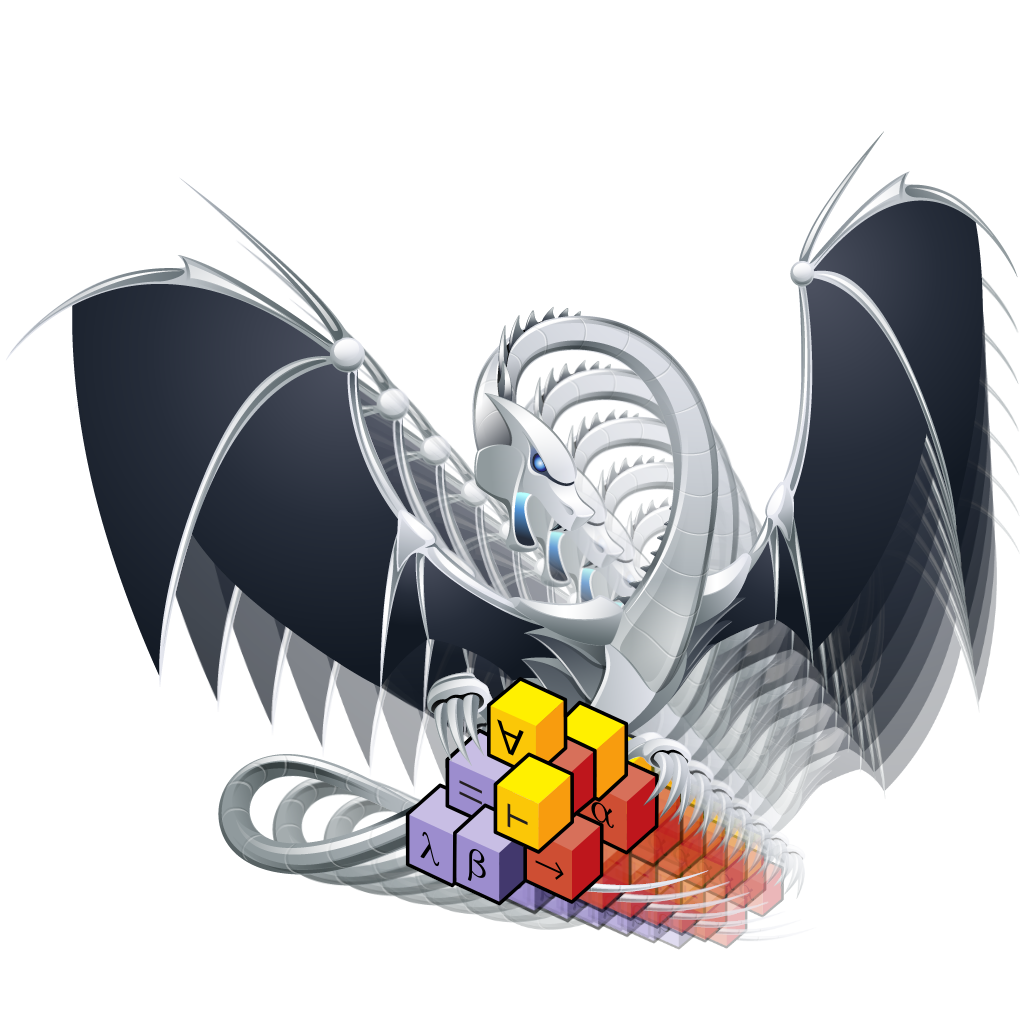
\includegraphics[width=.3\textwidth]{isabelle-llvm-par.png}};

    \path (a) -- (b) node[midway]{\huge\bfseries $\longrightarrow$};

  \end{tikzpicture}

%   {\small\center parallel combinator, separation logic, refine seq to par, refine lists to arrays}


\end{frame}
\begin{frame}[fragile]{Isabelle LLVM Back End}
  \begin{itemize}
   \item<+-> Shallow embedding into \only<4->{state-}\only<3->{ndet-}\only<2->{error-}monad \only<5->{with access reports}

  \end{itemize}
  \[\alpha~M =
    \only<2>{\alpha\textrm{ option}}
    \only<3>{\alpha \textrm{ set option}}
    \only<4>{\mu \to (\alpha\times\mu) \textrm{ set option} }
    \only<5->{\mu \to (\alpha\times\rho\times\mu) \textrm{ set option} }
  \]

  \onslide<2-> None --- undefined behaviour, nontermination

  \onslide<3-> $\alpha$ set --- set of possible results

  \onslide<4-> $\mu$ --- memory

  \onslide<5-> $\rho$ --- access report: read/written/allocated/freed addresses

  \onslide<6->

  \hfill

  Basic block: $x_1 \leftarrow op_1; \ldots; return \ldots$

  \onslide<7->

  if-then-else, while --- structured control flow (compiled by code-gen)

\end{frame}
\begin{frame}[t,fragile]{Parallel Operator}
  \newcommand{\mknd}[1]{\makebox[0pt]{\tikz[remember picture]{\node (#1) {};}}}

  \begin{itemize}
   \item<2-> $c_1 \parallel c_2$ --- execute in parallel, fail on data race
   \item<3-> Use access reports to detect data races

    \only<4>{
    \begin{tikzpicture}[node distance = 1cm, auto]
      \node (m) {$\mu$};
      \node[below left = of m] (m1) {$\rho_1,\mu_1$};
      \node[below right = of m] (m2) {$\rho_2,\mu_2$};
      \node[below right = of m1] (m') {};
      \node[above = 0mm of m',anchor=north] {$\rho',\mu'$};


      \draw[->] (m) -- node[swap] {\small $c_1$}  (m1);
      \draw[->] (m) -- node {\small $c_2$}  (m2);

      \draw[->] (m1) -- (m');
      \draw[->] (m2) -- (m');

      \node[above = .7em of m'] {\tiny combine};
      \node[above = 2em of m'] {\tiny check race};


    \end{tikzpicture}
    }


    \begin{onlyenv}<5-6>
    \begin{lstlisting}
      (c_1 || c_2) \mu ==
        (r_1,\rho$\mknd{r1}$_1,\mu_1) <- c_1 \mu --"\rightcomment{execute first strand}"
        (r_2,\rho$\mknd{r2}$_2,\mu_2) <- c_2 \mu --"\rightcomment{execute second strand}"
        assume \rho_1.alloc \<inter> \rho_2.alloc = \emptyset --"\rightcomment{ignore infeasible combinations}"
        assert no_race \rho_1 \rho_2 --"\rightcomment{fail on data race}"
        (\rho',\mu') = combine \rho_1 \mu_1   \rho_2 \mu_2 --"\rightcomment{combine states}"
        return ((r_1,r_2), \rho', \mu')
    \end{lstlisting}

    \onslide<6>
    Sanity checks: prove (as type invariant):
      \begin{itemize}
       \item access reports match actually modified addresses
       \item there is at least one execution.


%     \begin{lstlisting}
%       (c_1 || c_2) \mu ==
%         (r_1,\rho$\mknd{r1}$_1,\mu_1) <- c_1 \mu --"\rightcomment{execute first strand}"
%         (r_2,\rho$\mknd{r2}$_2,\mu_2) <- c_2 \mu --"\rightcomment{execute second strand}"
%         assert no_race \rho_1 \rho_2 --"\rightcomment{fail on data race}"
%         \mu' = combine \rho_1 \mu_1   \rho_2 \mu_2 --"\rightcomment{combine states}"
%         return ((r_1,r_2), \rho_1 \union \rho_2, \mu')
%
%     \end{lstlisting}

%     \begin{tikzpicture}[remember picture,overlay,ND/.style={anchor=west}]
%       \only<6->{
%       \node[ND,anchor=south] at ($(r1) + (3cm,-.1cm)$) (X) {\footnotesize Access report};
%       \draw (X) -- (r1);
%       \draw (X) -- (r2);
%       }
%     \end{tikzpicture}
      \end{itemize}
    \end{onlyenv}
   \item<7-> Code-gen: external function + some glue code
    \begin{onlyenv}<8->
    \small
    \begin{lstlisting}[language=C++]
    void parallel(void (*f1)(void*), void (*f2)(void*), void *x1, void *x2) {
      tbb::parallel_invoke([=]{f1(x1);}, [=]{f2(x2);});
    }
    \end{lstlisting}
    \end{onlyenv}


  \end{itemize}
\end{frame}
\begin{frame}[fragile]{Separation Logic}
  \begin{lstlisting}
    {P} c {Q} iff

      \<forall>\mu a af. \alpha \mu = a + af \and P a    --"\rightcomment{for all memories that satisfy precond}"
      ==> \<exists>S. c \mu = Some S                     --"\rightcomment{program does not fail}"
              \and \<forall>(r,\rho,\mu') \<in> S.       --"\rightcomment{and all possible results}"
                  \<exists> a'. \alpha \mu' = a'+af \and Q r a' --"\rightcomment{satisfy postcond}"
                  \and disjoint \rho af --"\rightcomment{and accessed memory not in frame}"

  \end{lstlisting}

  \lstinline{\alpha}: abstracts memory into separation algebra

  Baked-in frame rule

  \pause
  We prove the standard Hoare-rules, e.g.\ dj-conc rule:
  \begin{lstlisting}
    {P_1} c_1 {Q_1}   \and    {P_2} c_2 {Q_2}
    ==>
    {P_1 $\ast$ P_2} c_1 || c_2 {%(r_1,r_2). Q_1 r_1 $\ast$ Q_2 r_2}
  \end{lstlisting}

  \pause
  VCG helps with proof automation

\end{frame}
\begin{frame}[fragile]{Sepref}
  \begin{itemize}
   \item Semi-automatic data refinement.
    \begin{itemize}
     \item from purely functional nres-error monad
     \item to (shallowly embedded) LLVM semantics
     \item place pure data on heap (eg.\ lists $\to$ arrays)

    \end{itemize}
  \end{itemize}
\end{frame}
\begin{frame}[fragile]{Refinement Relation}

  \begin{lstlisting}
    hnr \Gamma c$_\dagger$ \Gamma' R CP c

    iff

    c=Some S ==> {\Gamma} c$_\dagger$ {%r$_\dagger$. \<exists>r. R r r$_\dagger$ $\ast$ \Gamma' $\ast$ r \<in> S $\ast$ CP r$_\dagger$}
  \end{lstlisting}

  \begin{itemize}
   \item[{$c_\dagger / c$}] concrete/abstract programs
   \item[{$\Gamma / \Gamma'$}] refinements for variables in $c_\dagger$ and $c$, before/after execution
   \item[{$R$}] refinement for result
   \item[{$CP$}] concrete (pointer) equalities

  \end{itemize}
  \onslide<2->
  \vfill

  Sepref: syntactically guided heuristics\\
    ~~~synthesize $c_\dagger$, $\Gamma'$, $R$, $CP$ from $\Gamma$ and $c$ + annotations


\end{frame}
\begin{frame}[fragile]{Example}
  \begin{lstlisting}
    hnr
      ( arr xs p $\ast$ idx n i ) --"\rightcomment{argument refinements}"
      ( store x (p+i); return p ) --"\rightcomment{concrete program: store, return pointer}"
      ( idx n i )                 --"\rightcomment{original refinement for array is gone}"
      ( arr )                     --"\rightcomment{result refinement}"
      ( %r. r=p )                 --"\rightcomment{concrete result is same as argument $p$}"
      ( return xs[n:=x] )         --"\rightcomment{abstract program: functional list update}"
  \end{lstlisting}

  \begin{itemize}
   \item[$arr$] refines list to array
   \item[$idx$] refines nat to size\_t


  \end{itemize}
\end{frame}
\begin{frame}{Refinement Building Blocks}
  \begin{itemize}
   \item<+-> Patterns and strategies for refinement
   \item<+-> Sequential: e.g., nat $\to$ size\_t, list $\to$ array, fold $\to$ loop
   \item<+-> Here: parallelization and array-splitting

  \end{itemize}
\end{frame}
\begin{frame}[fragile]{Parallelization}
  \begin{itemize}
   \item Refine sequential (independent) execution to parallel execution
    \small
    \begin{lstlisting}
      hnr \Gamma_1 c$_{\dagger1}$ \Gamma$_1'$ R_1 CP_1 c_1  \and   hnr \Gamma_2 c$_{\dagger2}$ \Gamma$_2'$ R_2 CP_2 c_2
      ==>
      hnr (\Gamma_1 $\ast$ \Gamma_2) (c$_{\dagger1}$ || c$_{\dagger2}$) (\Gamma$_1'$ $\ast$ \Gamma$_2'$) (R_1 \<times> R_2) (CP_1 \and CP_2) (fpar c_1 c_2)
    \end{lstlisting}

  \end{itemize}
  where
    \lstinline{fpar c_1 c_2 == r_1 <- c_1; r_2 <- c_2; return (r_1,r_2)}

    \lstinline{fpar} is annotation for Sepref to request parallelization

\end{frame}
\begin{frame}[fragile]{Array Splitting}
  \begin{itemize}
   \item Work on two separate parts of same array (e.g. in parallel)

   \item Functionally:
  \end{itemize}
  \begin{lstlisting}
    with_split n xs f =
      (xs_1,xs_2) <- f (take n xs) (drop n xs)
      return xs_1 @ xs_2
  \end{lstlisting}

  \begin{itemize}
   \item Imperative with arrays
  \end{itemize}
  \begin{lstlisting}
    with_split_arr i p f$_\dagger$ =
      p_2 <- ofs_ptr p i
      f$_\dagger$ p p_2
      return p
  \end{lstlisting}

  \begin{itemize}
   \item Refinement rule uses $CP$-predicates to ensure that $f_\dagger$ is in-place

  \end{itemize}
\end{frame}
\begin{frame}[fragile]{Parallel Quicksort}
  \begin{minipage}[t]{.49\textwidth}
  (Simplified) functional algorithm:
  \begin{lstlisting}
    qsort xs ==
      if |xs| < 1 then return xs
      else
        (xs,m) <- partition xs
        with_split m xs (%xs_1 xs_2.
          fpar (qsort xs_1) (qsort xs_2)
        )
  \end{lstlisting}
  \end{minipage}
  \begin{minipage}[t]{.49\textwidth}
  Correctness statement:
  \begin{lstlisting}
    qsort xs <= spec xs'. sorted xs'
                      \and mset xs' = mset xs
  \end{lstlisting}
  \end{minipage}

  \pause
  we have actually verified some 'extras':
  \begin{itemize}
   \item use sequential sorting for small, unbalanced, or deep partitions
   \item partitioning uses c=64 equidistant samples
   \item sequential sorting: using verified pdq-sort (competitive with std::sort)

  \end{itemize}
\end{frame}
\begin{frame}[fragile]{Correctness theorem and TCB}
  Sepref generates $qsort_\dagger$ and theorem

  \begin{lstlisting}
    hnr (arr xs p * idx |xs| n) (qsort$_\dagger$ p n) (idx |xs| n) arr (=p) (qsort xs)
  \end{lstlisting}

  \pause
  Combination with correctness theorem of $qsort$ yields

  \begin{lstlisting}
    {arr xs p * idx |xs| n}
      qsort$_\dagger$ p n
    {%r. \<exists>xs'. r=p $\ast$ arr xs' p $\ast$ sorted xs' $\ast$ mset xs' = mset xs}
  \end{lstlisting}

  \pause
  Code generator generates LLVM text from $qsort_\dagger$.

  \begin{lstlisting}
    export_llvm qsort$_\dagger$ is "uint64* qsort_uint64(uint64*, size_t)"
  \end{lstlisting}
  \vspace*{-.5em}
  (and, similar but more complicated for strings, ...)

  \pause
  \medskip
  This can be compiled and linked against, e.g., benchmark suite


\end{frame}
\begin{frame}{Benchmarks}

  \begin{tikzpicture}
    \begin{axis}[
      title={\large Laptop (6 core), uint64},
      ymajorgrids,
      title style={at={(0.2,.85)}},
      ybar=0pt,
      width=\textwidth,
      height=.85\textheight,
      bar width=3pt,
      xtick=data,
      symbolic x coords={rev-sorted-end-10,rev-sorted-end-1,sorted-end-.1,almost-sorted-50,random-boolean,organ-pipe,sorted-end-10,equal,rev-sorted-middle-.1,rev-sorted,sorted-middle-1,rev-sorted-middle-10,random,almost-sorted-.1,sorted,rev-sorted-middle-1,sorted-middle-.1,almost-sorted-10,almost-sorted-1,sorted-middle-10,rev-sorted-end-.1,sorted-end-1,random-dup-10,},
      xlabel near ticks, x tick label style={rotate=45,anchor=east,font=\tiny},
      legend style = {
%         legend pos= north east,
      at = {(.87,.97)},
%       cells={anchor=west},
      font=\scriptsize
      }
    ]
      \addplot[color=red,fill=red] coordinates {
(rev-sorted-end-10,895)
(rev-sorted-end-1,722)
(sorted-end-.1,373)
(almost-sorted-50,1032)
(random-boolean,717)
(organ-pipe,641)
(sorted-end-10,791)
(equal,706)
(rev-sorted-middle-.1,381)
(rev-sorted,614)
(sorted-middle-1,500)
(rev-sorted-middle-10,1024)
(random,1150)
(almost-sorted-.1,282)
(sorted,265)
(rev-sorted-middle-1,499)
(sorted-middle-.1,378)
(almost-sorted-10,705)
(almost-sorted-1,343)
(sorted-middle-10,992)
(rev-sorted-end-.1,681)
(sorted-end-1,451)
(random-dup-10,1100)
};
\addlegendentry{verified};
\addplot[color=blue,fill=blue] coordinates {
(rev-sorted-end-10,924)
(rev-sorted-end-1,857)
(sorted-end-.1,849)
(almost-sorted-50,1289)
(random-boolean,876)
(organ-pipe,866)
(sorted-end-10,942)
(equal,863)
(rev-sorted-middle-.1,864)
(rev-sorted,833)
(sorted-middle-1,892)
(rev-sorted-middle-10,1171)
(random,1438)
(almost-sorted-.1,873)
(sorted,855)
(rev-sorted-middle-1,896)
(sorted-middle-.1,857)
(almost-sorted-10,1038)
(almost-sorted-1,915)
(sorted-middle-10,1174)
(rev-sorted-end-.1,846)
(sorted-end-1,869)
(random-dup-10,1442)
};
\addlegendentry{std::sort};
\addplot[color=black,fill=black] coordinates {
(rev-sorted-end-10,851)
(rev-sorted-end-1,459)
(sorted-end-.1,363)
(almost-sorted-50,1049)
(random-boolean,975)
(organ-pipe,338)
(sorted-end-10,814)
(equal,72)
(rev-sorted-middle-.1,846)
(rev-sorted,115)
(sorted-middle-1,869)
(rev-sorted-middle-10,1094)
(random,1074)
(almost-sorted-.1,861)
(sorted,71)
(rev-sorted-middle-1,875)
(sorted-middle-.1,841)
(almost-sorted-10,926)
(almost-sorted-1,873)
(sorted-middle-10,1092)
(rev-sorted-end-.1,420)
(sorted-end-1,405)
(random-dup-10,1059)
};
\addlegendentry{sample sort};

    \end{axis}
  \end{tikzpicture}

\end{frame}
\begin{frame}{Benchmarks}

  \begin{tikzpicture}
    \begin{axis}[
      title={\large Laptop (6 core), string},
      ymajorgrids,
      title style={at={(0.2,.85)}},
      ybar=0pt,
      width=\textwidth,
      height=.85\textheight,
      bar width=3pt,
      xtick=data,
      symbolic x coords={rev-sorted-end-10,rev-sorted-end-1,sorted-end-.1,almost-sorted-50,random-boolean,organ-pipe,sorted-end-10,equal,rev-sorted-middle-.1,rev-sorted,sorted-middle-1,rev-sorted-middle-10,random,almost-sorted-.1,sorted,rev-sorted-middle-1,sorted-middle-.1,almost-sorted-10,almost-sorted-1,sorted-middle-10,rev-sorted-end-.1,sorted-end-1,random-dup-10,},
      xlabel near ticks, x tick label style={rotate=45,anchor=east,font=\tiny},
      legend style = {
%         legend pos= north east,
      at = {(.87,.97)},
%       cells={anchor=west},
      font=\scriptsize
      }
    ]
      \addplot[color=red,fill=red] coordinates {
(rev-sorted-end-10,637)
(rev-sorted-end-1,513)
(sorted-end-.1,469)
(almost-sorted-50,808)
(random-boolean,583)
(organ-pipe,563)
(sorted-end-10,587)
(equal,306)
(rev-sorted-middle-.1,518)
(rev-sorted,478)
(sorted-middle-1,494)
(rev-sorted-middle-10,678)
(random,870)
(almost-sorted-.1,427)
(sorted,347)
(rev-sorted-middle-1,532)
(sorted-middle-.1,474)
(almost-sorted-10,606)
(almost-sorted-1,445)
(sorted-middle-10,686)
(rev-sorted-end-.1,501)
(sorted-end-1,477)
(random-dup-10,910)
};
\addlegendentry{verified};
\addplot[color=gray,fill=gray] coordinates {
(rev-sorted-end-10,660)
(rev-sorted-end-1,558)
(sorted-end-.1,530)
(almost-sorted-50,823)
(random-boolean,989)
(organ-pipe,609)
(sorted-end-10,638)
(equal,470)
(rev-sorted-middle-.1,546)
(rev-sorted,509)
(sorted-middle-1,536)
(rev-sorted-middle-10,720)
(random,952)
(almost-sorted-.1,483)
(sorted,415)
(rev-sorted-middle-1,572)
(sorted-middle-.1,523)
(almost-sorted-10,630)
(almost-sorted-1,491)
(sorted-middle-10,695)
(rev-sorted-end-.1,552)
(sorted-end-1,521)
(random-dup-10,980)
};
\addlegendentry{verified-old};
\addplot[color=blue,fill=blue] coordinates {
(rev-sorted-end-10,404)
(rev-sorted-end-1,320)
(sorted-end-.1,290)
(almost-sorted-50,955)
(random-boolean,451)
(organ-pipe,295)
(sorted-end-10,403)
(equal,340)
(rev-sorted-middle-.1,299)
(rev-sorted,265)
(sorted-middle-1,407)
(rev-sorted-middle-10,689)
(random,1019)
(almost-sorted-.1,320)
(sorted,271)
(rev-sorted-middle-1,413)
(sorted-middle-.1,298)
(almost-sorted-10,660)
(almost-sorted-1,442)
(sorted-middle-10,667)
(rev-sorted-end-.1,286)
(sorted-end-1,318)
(random-dup-10,1028)
};
\addlegendentry{std::sort};
\addplot[color=black,fill=black] coordinates {
(rev-sorted-end-10,514)
(rev-sorted-end-1,322)
(sorted-end-.1,228)
(almost-sorted-50,866)
(random-boolean,711)
(organ-pipe,192)
(sorted-end-10,466)
(equal,150)
(rev-sorted-middle-.1,520)
(rev-sorted,281)
(sorted-middle-1,530)
(rev-sorted-middle-10,679)
(random,984)
(almost-sorted-.1,504)
(sorted,93)
(rev-sorted-middle-1,550)
(sorted-middle-.1,504)
(almost-sorted-10,614)
(almost-sorted-1,523)
(sorted-middle-10,644)
(rev-sorted-end-.1,316)
(sorted-end-1,255)
(random-dup-10,1003)
};
\addlegendentry{sample sort};

    \end{axis}
  \end{tikzpicture}

\end{frame}
\begin{frame}{Benchmarks}

  \begin{tikzpicture}
    \begin{axis}[
      title={\large Server (22 core), uint64},
      ymajorgrids,
      title style={at={(0.2,.85)}},
      ybar=0pt,
      width=\textwidth,
      height=.85\textheight,
      bar width=3pt,
      xtick=data,
      symbolic x coords={rev-sorted-end-10,rev-sorted-end-1,sorted-end-.1,almost-sorted-50,random-boolean,organ-pipe,sorted-end-10,equal,rev-sorted-middle-.1,rev-sorted,sorted-middle-1,rev-sorted-middle-10,random,almost-sorted-.1,sorted,rev-sorted-middle-1,sorted-middle-.1,almost-sorted-10,almost-sorted-1,sorted-middle-10,rev-sorted-end-.1,sorted-end-1,random-dup-10,},
      xlabel near ticks, x tick label style={rotate=45,anchor=east,font=\tiny},
      legend style = {
%         legend pos= north east,
      at = {(.87,.97)},
%       cells={anchor=west},
      font=\scriptsize
      }
    ]
      \addplot[color=red,fill=red] coordinates {
(rev-sorted-end-10,513)
(rev-sorted-end-1,334)
(sorted-end-.1,288)
(almost-sorted-50,895)
(random-boolean,670)
(organ-pipe,369)
(sorted-end-10,488)
(equal,402)
(rev-sorted-middle-.1,279)
(rev-sorted,280)
(sorted-middle-1,339)
(rev-sorted-middle-10,642)
(random,1072)
(almost-sorted-.1,240)
(sorted,244)
(rev-sorted-middle-1,340)
(sorted-middle-.1,287)
(almost-sorted-10,445)
(almost-sorted-1,262)
(sorted-middle-10,636)
(rev-sorted-end-.1,291)
(sorted-end-1,331)
(random-dup-10,1058)
};
\addlegendentry{verified};
\addplot[color=blue,fill=blue] coordinates {
(rev-sorted-end-10,609)
(rev-sorted-end-1,538)
(sorted-end-.1,536)
(almost-sorted-50,763)
(random-boolean,540)
(organ-pipe,543)
(sorted-end-10,613)
(equal,523)
(rev-sorted-middle-.1,544)
(rev-sorted,524)
(sorted-middle-1,589)
(rev-sorted-middle-10,776)
(random,837)
(almost-sorted-.1,554)
(sorted,533)
(rev-sorted-middle-1,592)
(sorted-middle-.1,544)
(almost-sorted-10,649)
(almost-sorted-1,592)
(sorted-middle-10,773)
(rev-sorted-end-.1,530)
(sorted-end-1,551)
(random-dup-10,849)
};
\addlegendentry{std::sort(par-unseq)};
\addplot[color=black,fill=black] coordinates {
(rev-sorted-end-10,398)
(rev-sorted-end-1,348)
(sorted-end-.1,268)
(almost-sorted-50,723)
(random-boolean,853)
(organ-pipe,240)
(sorted-end-10,370)
(equal,82)
(rev-sorted-middle-.1,529)
(rev-sorted,171)
(sorted-middle-1,574)
(rev-sorted-middle-10,724)
(random,746)
(almost-sorted-.1,538)
(sorted,75)
(rev-sorted-middle-1,578)
(sorted-middle-.1,544)
(almost-sorted-10,622)
(almost-sorted-1,562)
(sorted-middle-10,752)
(rev-sorted-end-.1,303)
(sorted-end-1,311)
(random-dup-10,766)
};
\addlegendentry{sample sort};

    \end{axis}
  \end{tikzpicture}

\end{frame}
\begin{frame}{Benchmarks}

  \begin{tikzpicture}
    \begin{axis}[
      title={\large Server (22 core), string},
      ymajorgrids,
      title style={at={(0.2,.85)}},
      ybar=0pt,
      width=\textwidth,
      height=.85\textheight,
      bar width=3pt,
      xtick=data,
      symbolic x coords={rev-sorted-end-10,rev-sorted-end-1,sorted-end-.1,almost-sorted-50,random-boolean,organ-pipe,sorted-end-10,equal,rev-sorted-middle-.1,rev-sorted,sorted-middle-1,rev-sorted-middle-10,random,almost-sorted-.1,sorted,rev-sorted-middle-1,sorted-middle-.1,almost-sorted-10,almost-sorted-1,sorted-middle-10,rev-sorted-end-.1,sorted-end-1,random-dup-10,},
      xlabel near ticks, x tick label style={rotate=45,anchor=east,font=\tiny},
      legend style = {
%         legend pos= north east,
      at = {(.87,.97)},
%       cells={anchor=west},
      font=\scriptsize
      }
    ]
      \addplot[color=red,fill=red] coordinates {
(rev-sorted-end-10,469)
(rev-sorted-end-1,400)
(sorted-end-.1,370)
(almost-sorted-50,520)
(random-boolean,906)
(organ-pipe,425)
(sorted-end-10,449)
(equal,521)
(rev-sorted-middle-.1,391)
(rev-sorted,378)
(sorted-middle-1,380)
(rev-sorted-middle-10,495)
(random,598)
(almost-sorted-.1,334)
(sorted,307)
(rev-sorted-middle-1,397)
(sorted-middle-.1,371)
(almost-sorted-10,411)
(almost-sorted-1,347)
(sorted-middle-10,472)
(rev-sorted-end-.1,387)
(sorted-end-1,377)
(random-dup-10,599)
};
\addlegendentry{verified};
\addplot[color=blue,fill=blue] coordinates {
(rev-sorted-end-10,205)
(rev-sorted-end-1,170)
(sorted-end-.1,161)
(almost-sorted-50,447)
(random-boolean,232)
(organ-pipe,174)
(sorted-end-10,207)
(equal,173)
(rev-sorted-middle-.1,165)
(rev-sorted,152)
(sorted-middle-1,214)
(rev-sorted-middle-10,335)
(random,465)
(almost-sorted-.1,175)
(sorted,155)
(rev-sorted-middle-1,213)
(sorted-middle-.1,165)
(almost-sorted-10,324)
(almost-sorted-1,230)
(sorted-middle-10,335)
(rev-sorted-end-.1,160)
(sorted-end-1,172)
(random-dup-10,508)
};
\addlegendentry{std::sort(par-unseq)};
\addplot[color=black,fill=black] coordinates {
(rev-sorted-end-10,284)
(rev-sorted-end-1,219)
(sorted-end-.1,201)
(almost-sorted-50,453)
(random-boolean,618)
(organ-pipe,166)
(sorted-end-10,272)
(equal,156)
(rev-sorted-middle-.1,261)
(rev-sorted,171)
(sorted-middle-1,274)
(rev-sorted-middle-10,395)
(random,508)
(almost-sorted-.1,244)
(sorted,108)
(rev-sorted-middle-1,295)
(sorted-middle-.1,232)
(almost-sorted-10,340)
(almost-sorted-1,255)
(sorted-middle-10,352)
(rev-sorted-end-.1,203)
(sorted-end-1,211)
(random-dup-10,518)
};
\addlegendentry{sample sort};

    \end{axis}
  \end{tikzpicture}

\end{frame}
\begin{frame}{Speedup}
  \begin{tikzpicture}
    \begin{axis}[
      xlabel near ticks,
      legend style = {
        at = {(.87,.3)},
        cells={anchor=west},
        font=\scriptsize
      },
      ymajorgrids,
      title={\large Laptop},
      title style={at={(0.15,.85)}},
      width=\textwidth,
      height=\textheight
    ]
      
\addplot+[color=red, mark color=black, mark options={fill=red}] coordinates {
  (1, 1.00)
  (2, 1.80)
  (3, 2.45)
  (4, 2.96)
  (5, 3.25)
  (6, 3.48)
  (7, 3.61)
  (8, 3.69)
  (9, 3.77)
  (10, 3.92)
  (11, 4.00)
  (12, 4.10)
};
\addlegendentry{verified};

\addplot+[color=black, mark color=black, mark options={fill=black}] coordinates {
  (1, 1.00)
  (2, 1.91)
  (3, 2.69)
  (4, 3.43)
  (5, 4.03)
  (6, 4.29)
  (7, 4.42)
  (8, 4.53)
  (9, 4.62)
  (10, 4.72)
  (11, 4.74)
  (12, 4.80)
};
\addlegendentry{sample sort};

\addplot+[color=blue, mark color=black, mark options={fill=blue}] coordinates {
  (1, 1.00)
  (2, 1.78)
  (3, 2.42)
  (4, 2.98)
  (5, 3.26)
  (6, 3.48)
  (7, 3.59)
  (8, 3.75)
  (9, 3.93)
  (10, 3.97)
  (11, 4.16)
  (12, 4.23)
};
\addlegendentry{std::sort(par-unseq)};


      \draw[black, thin, sharp plot]
      (axis cs:\pgfkeysvalueof{/pgfplots/xmin},\pgfkeysvalueof{/pgfplots/xmin}) --
      (axis cs:\pgfkeysvalueof{/pgfplots/xmax},\pgfkeysvalueof{/pgfplots/xmax});

%       \addplot[black, thin, sharp plot, update limits=false] {\x};
    \end{axis}
  \end{tikzpicture}

\end{frame}
\begin{frame}{Speedup}
  \begin{tikzpicture}
    \begin{axis}[
      xlabel near ticks,
      legend style = {
        at = {(.87,.3)},
        cells={anchor=west},
        font=\scriptsize
      },
      ymajorgrids,
      title={\large Server},
      title style={at={(0.15,.85)}},
      width=\textwidth,
      height=\textheight
    ]
      
\addplot+[color=red, mark color=black, mark options={fill=red}] coordinates {
  (1, 1.00)
  (2, 1.84)
  (3, 2.45)
  (4, 3.03)
  (5, 3.47)
  (6, 3.84)
  (7, 4.13)
  (8, 4.37)
  (9, 4.61)
  (10, 4.85)
  (11, 5.05)
  (12, 5.21)
  (13, 5.37)
  (14, 5.55)
  (15, 5.66)
  (16, 5.78)
  (17, 5.77)
  (18, 5.96)
  (19, 6.06)
  (20, 6.11)
  (21, 6.19)
  (22, 6.22)
};
\addlegendentry{verified};

\addplot+[color=black, mark color=black, mark options={fill=black}] coordinates {
  (1, 1.00)
  (2, 1.93)
  (3, 2.75)
  (4, 3.55)
  (5, 4.29)
  (6, 4.80)
  (7, 5.23)
  (8, 5.94)
  (9, 6.54)
  (10, 6.98)
  (11, 7.32)
  (12, 8.02)
  (13, 8.51)
  (14, 8.84)
  (15, 8.38)
  (16, 8.58)
  (17, 9.13)
  (18, 9.05)
  (19, 9.14)
  (20, 9.69)
  (21, 10.00)
  (22, 9.60)
};
\addlegendentry{sample sort};

\addplot+[color=blue, mark color=black, mark options={fill=blue}] coordinates {
  (1, 1.00)
  (2, 1.88)
  (3, 2.64)
  (4, 3.38)
  (5, 4.03)
  (6, 4.65)
  (7, 5.21)
  (8, 5.71)
  (9, 6.13)
  (10, 6.67)
  (11, 7.08)
  (12, 7.43)
  (13, 7.84)
  (14, 8.16)
  (15, 8.29)
  (16, 8.58)
  (17, 8.81)
  (18, 8.98)
  (19, 9.18)
  (20, 9.20)
  (21, 9.46)
  (22, 9.63)
};
\addlegendentry{std::sort(par-unseq)};


      \draw[black, thin, sharp plot]
      (axis cs:\pgfkeysvalueof{/pgfplots/xmin},\pgfkeysvalueof{/pgfplots/xmin}) --
      (axis cs:\pgfkeysvalueof{/pgfplots/xmax},\pgfkeysvalueof{/pgfplots/xmax});

%       \addplot[black, thin, sharp plot, update limits=false] {\x};
    \end{axis}
  \end{tikzpicture}

\end{frame}
\begin{frame}{Benchmark Interpretation}
  \begin{itemize}
   \item our algorithm is competitive for integers
   \item still some problems for strings
   \item could scale better to larger number of cores


  \end{itemize}
\end{frame}
{
\usebackgroundtemplate{%
\tikz\node[opacity=0.1] {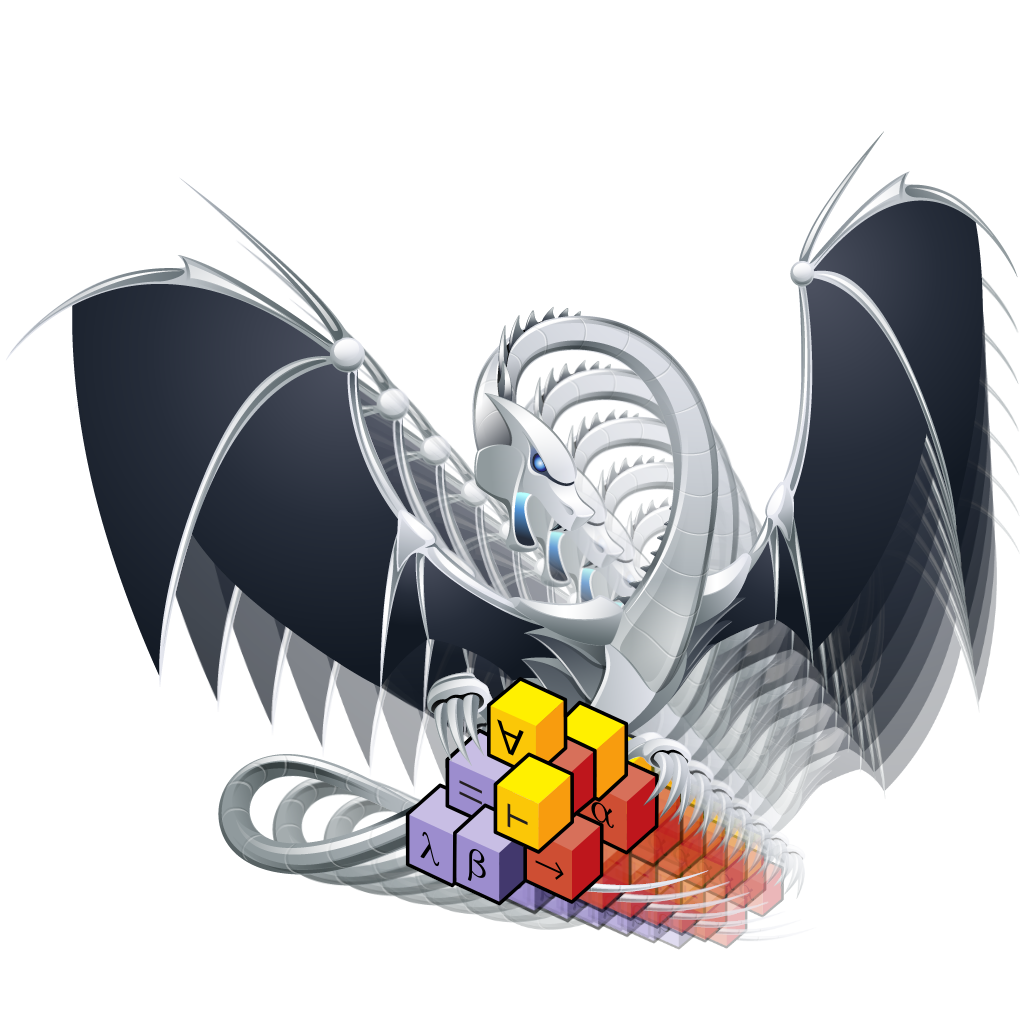
\includegraphics[height=\paperheight]{isabelle-llvm-par.png}};
}

\begin{frame}{Conclusion}
  \begin{itemize}
   \item Verification of parallel programs
    \begin{itemize}
     \item stepwise refinement to tackle complexity
     \item down to LLVM, small TCB
     \item \high{fast} verified programs

    \end{itemize}
   \item Idea: shallow embedding, using access reports
    \begin{itemize}
     \item backwards compatible with sequential IRF

    \end{itemize}
   \item Future work
    \begin{itemize}
     \item state-of-the-art parallel sorting
     \item fractional separation logic (for shared read-only)
     \item more concurrency (synchronization, atomic, ...)
     \item complexity of parallel algorithms
     \item GP-GPUs

    \end{itemize}
  \end{itemize}
  \vfill
  \url{https://www21.in.tum.de/~lammich/isabelle_llvm_par/}

  \url{https://github.com/lammich/isabelle_llvm/tree/2021-1}


\end{frame}
}



%   $\parallel$, $\frac{ \{P_1\} c_1 \{Q_1\}~~\{P_2\} c_2 \{Q_2\} }{\{P_1 \ast P_2\} c_1 \parallel c_2 \{Q_1 \ast Q_2\}}$, $\parallel \sqsubseteq \fatsemi$




% {
%
% \usebackgroundtemplate{%
% \only<3->{
% \tikz\node[opacity=0.1] {
\includegraphics[height=\paperheight]{isabelle-llvm.png}};
% }
% \only<2>{
% \tikz\node[opacity=1] {
\includegraphics[height=\paperheight]{isabelle-llvm.png}};
% }
% }
%
%
% #! Isabelle LLVM Back End
%   *<2-> Shallow embedding of small fragment of LLVM
%     * just enough to express our programs
%     * code generator translates to actual LLVM text
%   *<3-> Simple memory model {\small
%     \begin{lstlisting}
%       datatype addr == ADDR (bidx: nat) (idx: nat)
%       datatype ptr == PTR_NULL   |   PTR_ADDR (the_addr: addr)
%       datatype val == LL_INT lint   |   LL_STRUCT val list   |   LL_PTR ptr
%
%       datatype block == FRESH   |   FREED   |   is_alloc: ALLOC (vals: "val list")
%       typedef memory == { \mu :: nat => block. finite {b. \mu b ~= FRESH} }
%     \end{lstlisting}}
%
%   *<4-> Using state-error monad
%     \begin{lstlisting}
%       \alpha llM = memory => (FAIL | SUCC (\alpha \x memory))
%     \end{lstlisting}
%
%
%
%
% }
%
%
% #! Shallow Embedding Example
%   \newcommand{\mknd}[1]{\makebox[0pt]{\tikz[remember picture]{\node (#1) {};}}}
%   {\small\centering
%   \begin{minipage}[t]{.35\textwidth}
%     \begin{lstlisting}[escapechar=!]
%       fib:: 64 word !\mknd{ndparams}!=> 64 word ll!\mknd{ndrettype}!M
%       fib n = do {
%         t <- ll_icmp_ule n 1;
%         llc_if!\mknd{stmtif}! t
%           (return n)
%           (do {
%             n_1 <- ll_sub!\mknd{stmtsub}! n 1;
%             a   <- fib!\mknd{stmtrec}! n_1;
%             n_2 <- ll_sub n!\mknd{ndargs}! 2;
%             b   <-!\mknd{ndbind}! fib n_2;
%             c   <- ll_add a b;
%             return!\mknd{ndreturn}! c
%           }) }
%     \end{lstlisting}
% %     \begin{tikzpicture}[remember picture,overlay,ND/.style={rectangle callout, anchor=west,draw , fill=red!50, callout absolute pointer={#1}}]
% %       \node[ND=(ndrettype.east),anchor=south] at ($(ndrettype.north) + (0,.5cm)$) {\footnotesize state/error monad};
% %       \pause
% %       \node[ND=(ndparams.east)] at ($(ndparams -| 6,0) + (0,.5cm)$) {\footnotesize parameter types: words, pointers, pairs};
% %       \pause
% %       \node[ND=(stmtif.east)] at ($(stmtif -| 6,0) + (0,.5cm)$) {\footnotesize control flow (if, [optional: while])};
% %       \pause
% %       \node[ND=(stmtsub.east)] at ($(stmtsub -| 6,0)+(0,.5cm)$) {\footnotesize standard instructions};
% %       \pause
% %       \node[ND=(stmtrec.east)] at ($(stmtrec -| 6,0)+(0,.5cm)$) {\footnotesize function calls};
% %       \pause
% %       \node[ND=(ndargs.east)] at ($(ndargs -| 6,0)+(0,.5cm)$) {\footnotesize arguments: variables and constants};
% %       \pause
% %       \node[ND=(ndbind.east)] at ($(ndbind -| 6,0)+(0,.5cm)$) {\footnotesize monad: bind, return};
% %     \end{tikzpicture}
%     \begin{tikzpicture}[remember picture,overlay,ND/.style={anchor=west}]
%       \pause
%       \node[ND,anchor=south] at ($(ndrettype.north) + (0,.5cm)$) (X) {\footnotesize state/error monad};
%       \draw (X) -- (ndrettype);
%
%       \pause
%       \node[ND] at ($(ndparams -| 6,0) + (0,.5cm)$) (X) {\footnotesize types: word, pointer, struct};
%       \draw (X.west) -- (ndparams);
%
%       \pause
%       \node[ND=(ndbind.east)] at ($(ndbind -| 6,0)+(0,.5cm)$) (X) {\footnotesize monad: bind, return};
%       \draw (X.west) -- (ndbind);
%       \draw (X.west) -- (ndreturn);
%
%       \pause
%       \node[ND=(stmtsub.east)] at ($(stmtsub -| 6,0)+(0,.5cm)$) (X) {\footnotesize standard instructions (\is{ll_<opcode>})};
%       \draw (X.west) -- (stmtsub);
%
%       \pause
%       \node[ND=(ndargs.east)] at ($(ndargs -| 6,0)+(0,.5cm)$) (X) {\footnotesize arguments: variables and constants};
%       \draw (X.west) -- (ndargs);
%
%       \pause
%       \node[ND=(stmtif.east)] at ($(stmtif -| 6,0) + (0,.5cm)$) (X) {\footnotesize control flow (if, [optional: while])};
%       \draw (X.west) -- (stmtif);
%
%       \pause
%       \node[ND=(stmtrec.east)] at ($(stmtrec -| 6,0)+(0,.5cm)$) (X) {\footnotesize function calls (rec.\ via fixp in ccpo)};
%       \draw (X.west) -- (stmtrec);
%
%     \end{tikzpicture}
%   \end{minipage}
%   }
%
%
% #! Code Generation
%   \uncover<2->{compiling control flow + pretty printing}
%
%   {\small\centering
%   \begin{minipage}[t]{.35\textwidth}
%     \begin{lstlisting}
%       fib:: 64 word => 64 word llM
%       fib n = do {
%         t <- ll_icmp_ule n 1;
%         llc_if t
%
%           (return n)
%           (do {
%             n_1 <- ll_sub n 1;
%             a   <- fib n_1;
%             n_2 <- ll_sub n 2;
%             b   <- fib n_2;
%             c   <- ll_add a b;
%             return c
%           }) }
%     \end{lstlisting}
%   \end{minipage}
%   % \hspace*{.04\textwidth}
%   \hfill\pause
%   \begin{minipage}[t]{.57\textwidth}
%     \begin{lstlisting}[language=LLVM, literate={}]
%     define i64 @fib(i64 %n) {
%       start:
%         %t = icmp ule i64 %n, 1
%         br i1 %t, label %then, label %else
%       then:
%         br label %ctd_if
%       else:
%         %n_1 = sub i64 %n, 1
%         %a    = call i64 @fib (i64 %n_1)
%         %n_2 = sub i64 %n, 2
%         %b    = call i64 @fib (i64 %n_2)
%         %c    = add i64 %a, %b
%         br label %ctd_if
%       ctd_if:
%         %x1a = phi i64 [%n,%then], [%c,%else]
%         ret i64 %x1a }
%     \end{lstlisting}
%   \end{minipage}
%   }
%
%
%
% #! Preprocessor
%   * Only restricted terms accepted by code generator
%     * good to keep code generation simple
%     * tedious to write manually
%   * Preprocessor transforms terms into restricted format
%     * proves equality (via Isabelle kernel)
%   * Motto: Keep TCB small, preprocessor makes it usable
%
%
% #! Example: Preprocessing Euclid's Algorithm
%   \small
%   \begin{lstlisting}
%   euclid :: 64 word => 64 word => 64 word
%   euclid a b = do {
%     (a,b) <- llc_while
%       (%(a,b) => ll_cmp (a ~= b))
%       (%(a,b) => if (a<=b) then return (a,b-a) else return (a-b,b))
%       (a,b);
%     return a }
%   \end{lstlisting}
%   \pause
%   preprocessor defines function \is{euclid_0} and proves
%   \begin{lstlisting}
%   euclid a b = do {
%       ab <- ll_insert_1 init a; ab <- ll_insert_2 ab b;
%       ab <- euclid_0 ab;
%       ll_extract_1 ab  }
%   euclid_0 s = do {
%     a <- ll_extract_1 s;
%     b <- ll_extract_2 s;
%     ctd <- ll_icmp_ne a b;
%     llc_if ctd do {...; euclid_0 ...} }
%   \end{lstlisting}
%
%
% #! Reasoning about LLVM Programs
%   *<+-> Separation Logic
%     \begin{lstlisting}
%       \<alpha> :: memory -> amemory :: sep_algebra
%       wp c Q s == \<exists>r s'. c s = SUCC r s' \and Q r (\<alpha> s')
%       {P} c {Q} == \<forall>F s. (P * F) (\<alpha> s) --> wp c (\<lambda>r s'. (Q r * F) s') s
%     \end{lstlisting}
%
%     * defined wrt.\ shallowly embedded semantics
%     * proof rules are proved theorems!
%
%   *<+-> Automation: VCG, frame inference, heuristics to discharge VCs
%     * these prove theorems!
%
%   *<+-> Basic Data Structures: signed/unsigned integers, Booleans, arrays
%
% # Sepref
%   * Semi-automatic translation of functional to imperative program
%   * Data refinement to imperative DS
%     * e.g. list to array
%   * Proves refinement theorem
%
% #! Example: Binary Search
%   \newcommand{\mknd}[1]{\makebox[0pt]{\tikz[remember picture]{\node (#1) {};}}}
%   \begin{lstlisting}
%     definition "bin_search xs x = do {
%       (l,h) <- while (bin_search$\mknd{invar}$_invar xs x)
%         (%(l,h). l<h)
%         (%(l,h). do {
%           ass$\mknd{assn}$ert (l<|xs| \<and> h<=|xs| \<and> l<=h);
%           let m = l +$\mknd{midc}$ (h-l) div 2;
%           if xs!m < x then return (m+1,h) else return (l,m)
%         })
%         (0,|xs|);
%       return l
%     }"
%   \end{lstlisting}
%
%   \onslide<2->
%
%   \begin{tikzpicture}[remember picture,overlay,ND/.style={anchor=west}]
%     \only<2->{
%     \node[ND,anchor=west] at ($(invar) + (.5cm,-.5cm)$) (X) {\footnotesize invariant annotation};
%     \draw (X.west) -- (invar);
%     }
%
%     \only<3->{
%     \node[ND,anchor=west] at ($(assn) + (3cm,-3cm)$) (X) {\footnotesize hint for subsequent refinement};
%     \draw (X.west) -- (assn);
%     }
%
%     \only<4->{
%     \node[ND,anchor=west] at ($(midc) + (2,-1cm)$) (X) {\footnotesize overflow-safe midpoint computation};
%     \draw (X.west) -- (midc);
%     }
%   \end{tikzpicture}
%
%   \onslide<5->
%
%   \begin{lstlisting}
%   lemma bin_search_correct:
%     sorted xs ==> bin_search xs x <= spec i. i=find_index (<=y) xs
%   \end{lstlisting}
%
% #! Example: Binary Search --- Refinement
%   \newcommand{\mknd}[1]{\makebox[0pt]{\tikz[remember picture]{\node (#1) {};}}}
%   \onslide<1->
%
%   \begin{lstlisting}[escapechar=!]
%   sepref_def bin_search$_\dagger$ is bin_search
%     :: "(array$_A$!\mknd{assn1}! int$_A^{64}$)$^k$ $$* (int!\mknd{assn2}!$_A^{64}$)$^k$ -> int!\mknd{assn3}!$_A^{64}$
%     unfolding bin_search_def
%     apply (rule hfref_with_rdomI,!\mknd{assn4}! annot_snat_const "64")
%     by sep!\mknd{auto}!ref
%   \end{lstlisting}
%   \onslide<2->
%
%   \begin{tikzpicture}[remember picture,overlay,ND/.style={anchor=west}]
%   \only<2-3>{
%     \only<2->{
%     \node[ND,anchor=south] at ($(assn1) + (4cm,-3cm)$) (X) {\footnotesize hints for data refinement};
%     \draw (X) -- (assn1);
%     \draw (X) -- (assn2);
%     \draw (X) -- (assn3);
%     \draw (X) -- (assn4);
%     }
%
%     \only<3->{
%     \node[ND] at ($(auto) + (0,-2cm)$) (X) {\footnotesize automatic synthesis + proof};
%     \draw (X.west) -- (auto);
%     }
%   }
%   \end{tikzpicture}
%
%   \onslide<4->
%   proves: \is{(bin_search$_\dagger$, bin_search) \<in> (array$_A$ int$_A^{64}$)$^k$ * int${_A^{64}}^k$ -> int$_A^{64}$}
%   \onslide<5->
%
%   Combination with \is{bin_search_correct} yields:
%   \begin{lstlisting}
%   theorem bin_search$_\dagger$_correct:
%     {(array$_A$ int$_A^{64}$ xs xs$_\dagger$ * int$_A^{64}$ x x$_\dagger$ * sorted xs)}
%       (bin_search$_\dagger$ xs$_\dagger$ x$_\dagger$)
%     {%i$_\dagger$. \<exists>i. array$_A$ int$_A^{64}$ xs xs$_\dagger$ * int$_A^{64}$ x x$_\dagger$ * int$_A^{64}$ i i$_\dagger$ * i=find_index (<=y) xs}
%   \end{lstlisting}
%
%
% #! Example: Binary Search --- Generated Code
%   \newcommand{\mknd}[1]{\makebox[0pt]{\tikz[remember picture]{\node (#1) {};}}}
%
%   \begin{lstlisting}[escapechar=!]
%   export_llvm bin_se!\mknd{isaconst}!arch$_\dagger$ is int64_t bin_!\mknd{csig}!search(larray_t, elem_t)
%   defines
%     typedef !\mknd{tdefs}!int64_t elem_t;
%     typedef struct { int64_t len; elem_t *data; } larray_t;
%   file "!\mknd{file}!code/bin_search.ll"
%   \end{lstlisting}
%
%
%   \begin{tikzpicture}[remember picture,overlay,ND/.style={anchor=west}]
%   \only<2-5>{
%     \only<2->{
%     \node[ND,anchor=south] at ($(isaconst) + (0,-3cm)$) (X) {\footnotesize Isabelle constant};
%     \draw (X) -- (isaconst);
%     }
%
%     \only<3->{
%     \node[ND] at ($(csig) + (0,-3cm)$) (X) {\footnotesize LLVM name and signature};
%     \draw (X.west) -- (csig);
%     }
%
%     \only<4->{
%     \node[ND] at ($(tdefs) + (0,-3cm)$) (X) {\footnotesize C-style typedefs};
%     \draw (X.west) -- (tdefs);
%     }
%
%     \only<5->{
%     \node[ND] at ($(file) + (0,-3cm)$) (X) {\footnotesize target file};
%     \draw (X.west) -- (file);
%     }
%   }
%   \end{tikzpicture}
%
%   \onslide<6->
%
%   Produces LLVM code and header file:
%   \begin{lstlisting}[language=C]
%     typedef int64_t elem_t;
%     typedef struct {
%       int64_t len;
%       elem_t*data;
%     } larray_t;
%
%     int64_t bin_search(larray_t,elem_t);
%   \end{lstlisting}
%
%
% {
% \usebackgroundtemplate{%
% \only<3->{
% \tikz\node[opacity=0.1] {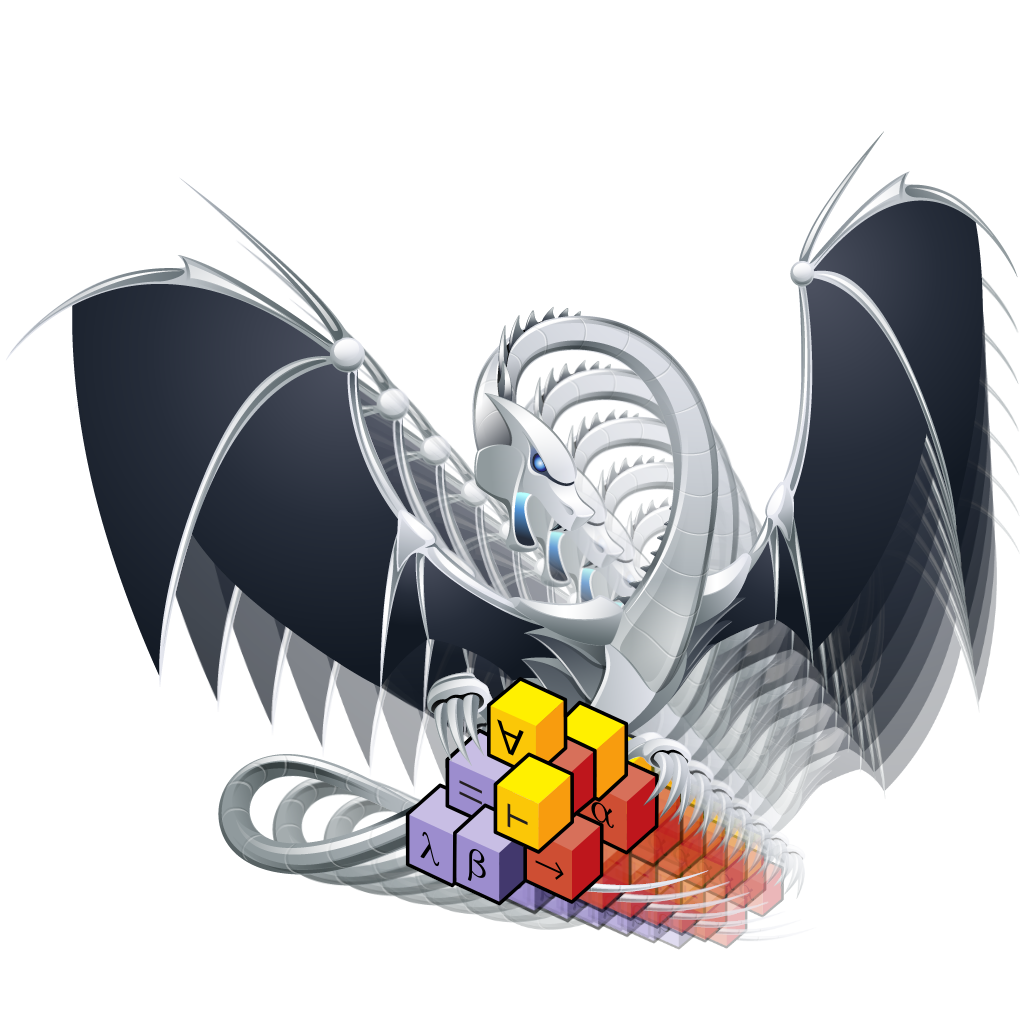
\includegraphics[height=\paperheight]{isabelle-llvm-par.png}};
% }
% \only<2>{
% \tikz\node[opacity=1] {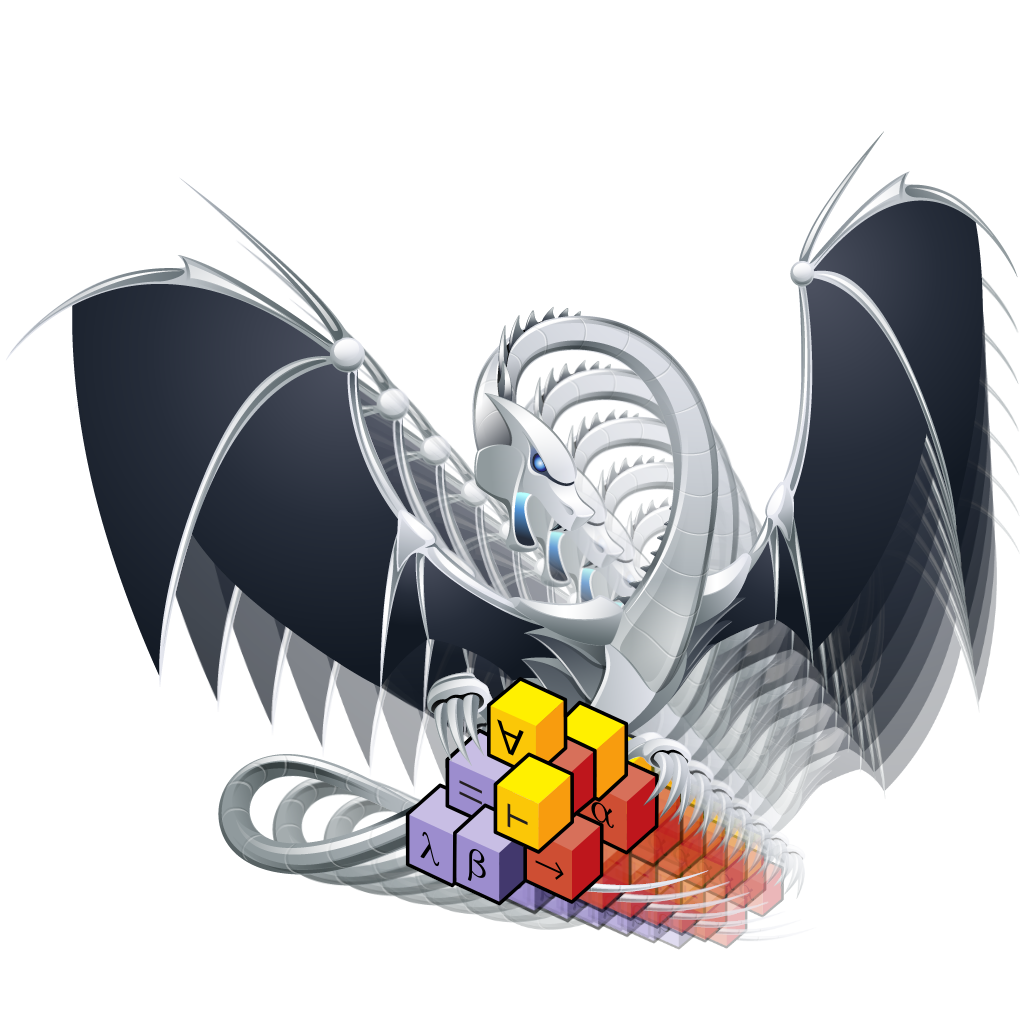
\includegraphics[height=\paperheight]{isabelle-llvm-par.png}};
% }
% }
%
% #![t] Isabelle-LLVM Parallel
%   \newcommand{\mknd}[1]{\makebox[0pt]{\tikz[remember picture]{\node (#1) {};}}}
%
%   *<2-> Add parallel operator: $c_1 \parallel c_2$
%     *<3-> execute in parallel, fail on data race
%   *<4-> Shallow embedding: make program report memory accesses
%
%     \only<4>{
%     \begin{tikzpicture}[node distance = 1cm, auto]
%       \node (m) {$\mu$};
%       \node[below left = of m] (m1) {$\rho_1,\mu_1$};
%       \node[below right = of m] (m2) {$\rho_2,\mu_2$};
%       \node[below right = of m1] (m') {$\mu'$};
%
%       \draw[->] (m) -- node[swap] {\small $c_1$}  (m1);
%       \draw[->] (m) -- node {\small $c_2$}  (m2);
%
%       \draw[->] (m1) -- (m');
%       \draw[->] (m2) -- (m');
%
%       \node[above = .7em of m'] {\tiny combine};
%       \node[above = 2em of m'] {\tiny check race};
%
%
%     \end{tikzpicture}
%     }
%
%
%     \begin{onlyenv}<5-6>
%     \begin{lstlisting}
%       (c_1 || c_2) \mu ==
%         (r_1,\rho$\mknd{r1}$_1,\mu_1) <- c_1 \mu --"\rightcomment{execute first strand}"
%         (r_2,\rho$\mknd{r2}$_2,\mu_2) <- c_2 \mu --"\rightcomment{execute second strand}"
%         assert no_race \rho_1 \rho_2 --"\rightcomment{fail on data race}"
%         \mu' = combine \rho_1 \mu_1   \rho_2 \mu_2 --"\rightcomment{combine states}"
%         return ((r_1,r_2), \rho_1 \union \rho_2, \mu')
%
%     \end{lstlisting}
%
%     \begin{tikzpicture}[remember picture,overlay,ND/.style={anchor=west}]
%       \only<6->{
%       \node[ND,anchor=south] at ($(r1) + (3cm,-.1cm)$) (X) {\footnotesize Access report};
%       \draw (X) -- (r1);
%       \draw (X) -- (r2);
%       }
%     \end{tikzpicture}
%     \end{onlyenv}
%
% }
%
% #! Memory Allocation
%   *<+-> Currently: deterministic semantics
%     * $c_1~\mu$ and $c_2~\mu$ will allocate same memory
%     * cannot be combined!
%
%   *<+-> Use nondeterminism
%     \begin{lstlisting}
%       \alpha llM = memory => FAIL | SUCC ((\alpha \x report \x memory) set)
%     \end{lstlisting}
%     * malloc nondeterministically allocates some free address
%     * on combination: exclude infeasible possibilities
%
%   \onslide<+->
%   \begin{lstlisting}
%     (c_1 || c_2) \mu ==
%       (r_1,\rho_1,\mu_1) <- c_1 \mu
%       (r_2,\rho_2,\mu_2) <- c_2 \mu
%       assume \rho_1.alloc \<inter> \rho_2.alloc = \emptyset --"\rightcomment{ignore infeasible combinations}"
%       assert no_race \rho_1 \rho_2 --"\rightcomment{fail on data race}"
%       \mu' = combine \rho_1 \mu_1   \rho_2 \mu_2 --"\rightcomment{combine states}"
%       return ((r_1,r_2), \rho_1 \union \rho_2, \mu')
%
%   \end{lstlisting}
%
% #! Invariants
%   * We prove for \is{llM} (enforced by subtype)
%     * access reports are consistent with observed changes in memory
%     * there is at least one possible result (no magic happens)
%
%   * Sanity check for semantics
%
%   * Allows us to prove symmetry of $\parallel$
%     \begin{lstlisting}
%       c_1 || c_2  =  swapres (c_2 || c_1)
%
%       swapres m == (r_1,r_2)<-m; return (r_2,r_1)
%     \end{lstlisting}
%
% #! Code generator
%   *<+-> We add \is{llc_par f_1 f_2 x_1 x_2 == f_1 x_1 || f_2 x_2}
%     * \is{f_1, f_2} must be functions
%   *<+-> Code generator generates
%     * type casting boilerplate
%     * call to external \is{parallel} function
%
%     {\small
%     \begin{lstlisting}[language=C++]
%     void parallel(void (*f1)(void*), void (*f2)(void*), void *x1, void *x2)
%     \end{lstlisting}
%     }
%   *<+-> For example, implemented using TBB:
%     {\small
%     \begin{lstlisting}[language=C++]
%     {
%       tbb::parallel_invoke([=]{f1(x1);}, [=]{f2(x2);});
%     }
%     \end{lstlisting}
%     }
%
%
%
% #! Amending higher layers of IRF
%   *<+-> Prove concurrency rule
%     \begin{lstlisting}
%       ${}$        {P_1} c_1 {Q_1}    \and    {P_2} c_2 {Q_2}
%     \end{lstlisting}
%
%     \vspace*{-.8em}
%     \begin{lstlisting}
%       ==> {P_1 * P_2} c_1 || c_2 {%(r_1,r_2). Q_1 r_1 * Q_2 r_2}
%     \end{lstlisting}
%
%   *<+-> Sepref refines sequential to parallel execution
%     \begin{lstlisting}
%       npar f_1 f_2 x_1 x_2 == r_1 <- f_1 x_1; r_2 <- f_2 x_2; return (r_1,r_2)
%     \end{lstlisting}
%     refined to \is{llc_par}.
%
%   *<+-> Backwards compatible with sequential Sepref!
%     * Easy porting of existing algorithms
%
% #! Parallel Quicksort (basic)
%
%   \begin{lstlisting}
%     psort xs ==
%       if |xs|<=1 then return xs    --"\rightcomment{trivially sorted}"
%       else
%         (xs,m) <- partition_spec xs;  --"\rightcomment{partition}"
%         (_,xs) <- with_split m xs (%xs_1 xs_2.
%           npar psort psort xs_1 xs_2 --"\rightcomment{recursively sort partitions}"
%         );
%         return xs
%
%     with_split i xs f ==
%       assert (i < |xs|);       --"\rightcomment{split point must be in list}"
%       (xs_1,xs_2) <- f (take i xs) (drop i xs); --"\rightcomment{execute f with halfs}"
%       assert (|xs_1| = i \and |xs_2| = |xs| - i); --"\rightcomment{length of halfs must not change}"
%       return (xs_1@xs_2) --"\rightcomment{return both halfs}"
%
%   \end{lstlisting}
%
%
% #! Parallel Quicksort (refined)
%   \small
%   \begin{lstlisting}
%     psort xs n ==
%       assert n=|xs|;
%       if n<=1 then return xs
%       else psort_aux xs n (log2 n * 2) --"\rightcomment{recursion depth limit}"
%
%     psort_aux xs n d ==
%       assert n=|xs|  --"\rightcomment{extra parameter for length}"
%       if d=0 \or n<100000 then sort_spec xs --"\rightcomment{fallback to seq-sort}"
%       else
%         (xs,m) <- partition_spec xs;
%         let bad = m<n div 8 \or (n-m < n div 8) --"\rightcomment{check unbalanced partition}"
%         (_,xs) <- with_split m xs (%xs_1 xs_2.
%           if bad then --"\rightcomment{sequentially recurse for unbalanced}"
%             nseq psort_aux psort_aux (xs_1,m,d-1) (xs_2,n-m,d-1)
%           else --"\rightcomment{recurse in parallel for balanced}"
%             npar psort_aux psort_aux (xs_1,m,d-1) (xs_2,n-m,d-1)
%         );
%         return xs"
%
%   \end{lstlisting}
%
% #![t] Parallel Quicksort (Sepref + Code Export)
%   \small
%
%   *<1-> Sepref generates imperative program
%     * using existing sequential \is{pdqsort} for fallback
%     * using (new) sampling partitioner (proved correct + refined separately)
%
%   *<2-> Correctness theorem:
%     {\only<3->{\tiny}
%     \begin{lstlisting}
%     {arr$_A$ xs xs$_\dagger$ * idx$_A$ n n$_\dagger$ * n = |xs|}
%       (psort$_\dagger$ xs$_\dagger$ n$_\dagger$)
%     {%r. r=xs$_\dagger$ * \<exists> xs'. arr$_A$ xs' xs$_\dagger$ * sorted xs' * mset xs' = mset xs}
%     \end{lstlisting}}
%   *<3-> Instantiation to concrete weak ordering + code export
%     {\only<4->{\tiny}
%     \begin{lstlisting}
%       interpretation unat: pcmp (%_. <) (%_. ll_icmp_ult) unat$^{64}_A$ \<proof>
%       interpretation str: pcmp (%_. <) (%_. strcmp) str$^{64}_A$ \<proof>
%
%       export_llvm
%         unat.psort$_\dagger$ is "uint64_t* psort(uint64_t*, int64_t)"
%         str.psort$_\dagger$ is "llstring* str_psort(llstring*, int64_t)"
%         defines
%           typedef struct {int64_t sz; struct {int64_t cap; char *data;};} llstring;
%         file psort.ll
%     \end{lstlisting}}
%
%   *<4-> Link against C++ benchmark driver
%     \begin{lstlisting}
%       clang++ [...] lib_isabelle_llvm.cpp psort.ll benchmark.cpp
%     \end{lstlisting}
%
% \tikzset{myaxis/.style={
%       ymajorgrids,
%       title style={at={(0.2,.85)}},
%       ybar=0pt,
%       width=\textwidth,
%       height=.85\textheight,
%       bar width=3pt,
%       xtick=data,
%       symbolic x coords={rev-sorted-end-10,rev-sorted-end-1,sorted-end-.1,almost-sorted-50,random-boolean,organ-pipe,sorted-end-10,equal,rev-sorted-middle-.1,rev-sorted,sorted-middle-1,rev-sorted-middle-10,random,almost-sorted-.1,sorted,rev-sorted-middle-1,sorted-middle-.1,almost-sorted-10,almost-sorted-1,sorted-middle-10,rev-sorted-end-.1,sorted-end-1,random-dup-10,},
%       xlabel near ticks, x tick label style={rotate=45,anchor=east,font=\tiny},
%       legend style = {
% %         legend pos= north east,
%       at = {(.87,.97)},
% %       cells={anchor=west},
%       font=\scriptsize
%       }
% }}
%
% # Benchmarks
%
%   \begin{tikzpicture}
%     \begin{axis}[
%       title={\large Laptop (6 core), uint64},
%       ymajorgrids,
%       title style={at={(0.2,.85)}},
%       ybar=0pt,
%       width=\textwidth,
%       height=.85\textheight,
%       bar width=3pt,
%       xtick=data,
%       symbolic x coords={rev-sorted-end-10,rev-sorted-end-1,sorted-end-.1,almost-sorted-50,random-boolean,organ-pipe,sorted-end-10,equal,rev-sorted-middle-.1,rev-sorted,sorted-middle-1,rev-sorted-middle-10,random,almost-sorted-.1,sorted,rev-sorted-middle-1,sorted-middle-.1,almost-sorted-10,almost-sorted-1,sorted-middle-10,rev-sorted-end-.1,sorted-end-1,random-dup-10,},
%       xlabel near ticks, x tick label style={rotate=45,anchor=east,font=\tiny},
%       legend style = {
% %         legend pos= north east,
%       at = {(.87,.97)},
% %       cells={anchor=west},
%       font=\scriptsize
%       }
%     ]
%       \addplot[color=red,fill=red] coordinates {
(rev-sorted-end-10,895)
(rev-sorted-end-1,722)
(sorted-end-.1,373)
(almost-sorted-50,1032)
(random-boolean,717)
(organ-pipe,641)
(sorted-end-10,791)
(equal,706)
(rev-sorted-middle-.1,381)
(rev-sorted,614)
(sorted-middle-1,500)
(rev-sorted-middle-10,1024)
(random,1150)
(almost-sorted-.1,282)
(sorted,265)
(rev-sorted-middle-1,499)
(sorted-middle-.1,378)
(almost-sorted-10,705)
(almost-sorted-1,343)
(sorted-middle-10,992)
(rev-sorted-end-.1,681)
(sorted-end-1,451)
(random-dup-10,1100)
};
\addlegendentry{verified};
\addplot[color=blue,fill=blue] coordinates {
(rev-sorted-end-10,924)
(rev-sorted-end-1,857)
(sorted-end-.1,849)
(almost-sorted-50,1289)
(random-boolean,876)
(organ-pipe,866)
(sorted-end-10,942)
(equal,863)
(rev-sorted-middle-.1,864)
(rev-sorted,833)
(sorted-middle-1,892)
(rev-sorted-middle-10,1171)
(random,1438)
(almost-sorted-.1,873)
(sorted,855)
(rev-sorted-middle-1,896)
(sorted-middle-.1,857)
(almost-sorted-10,1038)
(almost-sorted-1,915)
(sorted-middle-10,1174)
(rev-sorted-end-.1,846)
(sorted-end-1,869)
(random-dup-10,1442)
};
\addlegendentry{std::sort};
\addplot[color=black,fill=black] coordinates {
(rev-sorted-end-10,851)
(rev-sorted-end-1,459)
(sorted-end-.1,363)
(almost-sorted-50,1049)
(random-boolean,975)
(organ-pipe,338)
(sorted-end-10,814)
(equal,72)
(rev-sorted-middle-.1,846)
(rev-sorted,115)
(sorted-middle-1,869)
(rev-sorted-middle-10,1094)
(random,1074)
(almost-sorted-.1,861)
(sorted,71)
(rev-sorted-middle-1,875)
(sorted-middle-.1,841)
(almost-sorted-10,926)
(almost-sorted-1,873)
(sorted-middle-10,1092)
(rev-sorted-end-.1,420)
(sorted-end-1,405)
(random-dup-10,1059)
};
\addlegendentry{sample sort};

%     \end{axis}
%   \end{tikzpicture}
%
% # Benchmarks
%
%   \begin{tikzpicture}
%     \begin{axis}[
%       title={\large Laptop (6 core), string},
%       ymajorgrids,
%       title style={at={(0.2,.85)}},
%       ybar=0pt,
%       width=\textwidth,
%       height=.85\textheight,
%       bar width=3pt,
%       xtick=data,
%       symbolic x coords={rev-sorted-end-10,rev-sorted-end-1,sorted-end-.1,almost-sorted-50,random-boolean,organ-pipe,sorted-end-10,equal,rev-sorted-middle-.1,rev-sorted,sorted-middle-1,rev-sorted-middle-10,random,almost-sorted-.1,sorted,rev-sorted-middle-1,sorted-middle-.1,almost-sorted-10,almost-sorted-1,sorted-middle-10,rev-sorted-end-.1,sorted-end-1,random-dup-10,},
%       xlabel near ticks, x tick label style={rotate=45,anchor=east,font=\tiny},
%       legend style = {
% %         legend pos= north east,
%       at = {(.87,.97)},
% %       cells={anchor=west},
%       font=\scriptsize
%       }
%     ]
%       \addplot[color=red,fill=red] coordinates {
(rev-sorted-end-10,637)
(rev-sorted-end-1,513)
(sorted-end-.1,469)
(almost-sorted-50,808)
(random-boolean,583)
(organ-pipe,563)
(sorted-end-10,587)
(equal,306)
(rev-sorted-middle-.1,518)
(rev-sorted,478)
(sorted-middle-1,494)
(rev-sorted-middle-10,678)
(random,870)
(almost-sorted-.1,427)
(sorted,347)
(rev-sorted-middle-1,532)
(sorted-middle-.1,474)
(almost-sorted-10,606)
(almost-sorted-1,445)
(sorted-middle-10,686)
(rev-sorted-end-.1,501)
(sorted-end-1,477)
(random-dup-10,910)
};
\addlegendentry{verified};
\addplot[color=gray,fill=gray] coordinates {
(rev-sorted-end-10,660)
(rev-sorted-end-1,558)
(sorted-end-.1,530)
(almost-sorted-50,823)
(random-boolean,989)
(organ-pipe,609)
(sorted-end-10,638)
(equal,470)
(rev-sorted-middle-.1,546)
(rev-sorted,509)
(sorted-middle-1,536)
(rev-sorted-middle-10,720)
(random,952)
(almost-sorted-.1,483)
(sorted,415)
(rev-sorted-middle-1,572)
(sorted-middle-.1,523)
(almost-sorted-10,630)
(almost-sorted-1,491)
(sorted-middle-10,695)
(rev-sorted-end-.1,552)
(sorted-end-1,521)
(random-dup-10,980)
};
\addlegendentry{verified-old};
\addplot[color=blue,fill=blue] coordinates {
(rev-sorted-end-10,404)
(rev-sorted-end-1,320)
(sorted-end-.1,290)
(almost-sorted-50,955)
(random-boolean,451)
(organ-pipe,295)
(sorted-end-10,403)
(equal,340)
(rev-sorted-middle-.1,299)
(rev-sorted,265)
(sorted-middle-1,407)
(rev-sorted-middle-10,689)
(random,1019)
(almost-sorted-.1,320)
(sorted,271)
(rev-sorted-middle-1,413)
(sorted-middle-.1,298)
(almost-sorted-10,660)
(almost-sorted-1,442)
(sorted-middle-10,667)
(rev-sorted-end-.1,286)
(sorted-end-1,318)
(random-dup-10,1028)
};
\addlegendentry{std::sort};
\addplot[color=black,fill=black] coordinates {
(rev-sorted-end-10,514)
(rev-sorted-end-1,322)
(sorted-end-.1,228)
(almost-sorted-50,866)
(random-boolean,711)
(organ-pipe,192)
(sorted-end-10,466)
(equal,150)
(rev-sorted-middle-.1,520)
(rev-sorted,281)
(sorted-middle-1,530)
(rev-sorted-middle-10,679)
(random,984)
(almost-sorted-.1,504)
(sorted,93)
(rev-sorted-middle-1,550)
(sorted-middle-.1,504)
(almost-sorted-10,614)
(almost-sorted-1,523)
(sorted-middle-10,644)
(rev-sorted-end-.1,316)
(sorted-end-1,255)
(random-dup-10,1003)
};
\addlegendentry{sample sort};

%     \end{axis}
%   \end{tikzpicture}
%
% # Benchmarks
%
%   \begin{tikzpicture}
%     \begin{axis}[
%       title={\large Server (22 core), uint64},
%       ymajorgrids,
%       title style={at={(0.2,.85)}},
%       ybar=0pt,
%       width=\textwidth,
%       height=.85\textheight,
%       bar width=3pt,
%       xtick=data,
%       symbolic x coords={rev-sorted-end-10,rev-sorted-end-1,sorted-end-.1,almost-sorted-50,random-boolean,organ-pipe,sorted-end-10,equal,rev-sorted-middle-.1,rev-sorted,sorted-middle-1,rev-sorted-middle-10,random,almost-sorted-.1,sorted,rev-sorted-middle-1,sorted-middle-.1,almost-sorted-10,almost-sorted-1,sorted-middle-10,rev-sorted-end-.1,sorted-end-1,random-dup-10,},
%       xlabel near ticks, x tick label style={rotate=45,anchor=east,font=\tiny},
%       legend style = {
% %         legend pos= north east,
%       at = {(.87,.97)},
% %       cells={anchor=west},
%       font=\scriptsize
%       }
%     ]
%       \addplot[color=red,fill=red] coordinates {
(rev-sorted-end-10,513)
(rev-sorted-end-1,334)
(sorted-end-.1,288)
(almost-sorted-50,895)
(random-boolean,670)
(organ-pipe,369)
(sorted-end-10,488)
(equal,402)
(rev-sorted-middle-.1,279)
(rev-sorted,280)
(sorted-middle-1,339)
(rev-sorted-middle-10,642)
(random,1072)
(almost-sorted-.1,240)
(sorted,244)
(rev-sorted-middle-1,340)
(sorted-middle-.1,287)
(almost-sorted-10,445)
(almost-sorted-1,262)
(sorted-middle-10,636)
(rev-sorted-end-.1,291)
(sorted-end-1,331)
(random-dup-10,1058)
};
\addlegendentry{verified};
\addplot[color=blue,fill=blue] coordinates {
(rev-sorted-end-10,609)
(rev-sorted-end-1,538)
(sorted-end-.1,536)
(almost-sorted-50,763)
(random-boolean,540)
(organ-pipe,543)
(sorted-end-10,613)
(equal,523)
(rev-sorted-middle-.1,544)
(rev-sorted,524)
(sorted-middle-1,589)
(rev-sorted-middle-10,776)
(random,837)
(almost-sorted-.1,554)
(sorted,533)
(rev-sorted-middle-1,592)
(sorted-middle-.1,544)
(almost-sorted-10,649)
(almost-sorted-1,592)
(sorted-middle-10,773)
(rev-sorted-end-.1,530)
(sorted-end-1,551)
(random-dup-10,849)
};
\addlegendentry{std::sort(par-unseq)};
\addplot[color=black,fill=black] coordinates {
(rev-sorted-end-10,398)
(rev-sorted-end-1,348)
(sorted-end-.1,268)
(almost-sorted-50,723)
(random-boolean,853)
(organ-pipe,240)
(sorted-end-10,370)
(equal,82)
(rev-sorted-middle-.1,529)
(rev-sorted,171)
(sorted-middle-1,574)
(rev-sorted-middle-10,724)
(random,746)
(almost-sorted-.1,538)
(sorted,75)
(rev-sorted-middle-1,578)
(sorted-middle-.1,544)
(almost-sorted-10,622)
(almost-sorted-1,562)
(sorted-middle-10,752)
(rev-sorted-end-.1,303)
(sorted-end-1,311)
(random-dup-10,766)
};
\addlegendentry{sample sort};

%     \end{axis}
%   \end{tikzpicture}
%
% # Benchmarks
%
%   \begin{tikzpicture}
%     \begin{axis}[
%       title={\large Server (22 core), string},
%       ymajorgrids,
%       title style={at={(0.2,.85)}},
%       ybar=0pt,
%       width=\textwidth,
%       height=.85\textheight,
%       bar width=3pt,
%       xtick=data,
%       symbolic x coords={rev-sorted-end-10,rev-sorted-end-1,sorted-end-.1,almost-sorted-50,random-boolean,organ-pipe,sorted-end-10,equal,rev-sorted-middle-.1,rev-sorted,sorted-middle-1,rev-sorted-middle-10,random,almost-sorted-.1,sorted,rev-sorted-middle-1,sorted-middle-.1,almost-sorted-10,almost-sorted-1,sorted-middle-10,rev-sorted-end-.1,sorted-end-1,random-dup-10,},
%       xlabel near ticks, x tick label style={rotate=45,anchor=east,font=\tiny},
%       legend style = {
% %         legend pos= north east,
%       at = {(.87,.97)},
% %       cells={anchor=west},
%       font=\scriptsize
%       }
%     ]
%       \addplot[color=red,fill=red] coordinates {
(rev-sorted-end-10,469)
(rev-sorted-end-1,400)
(sorted-end-.1,370)
(almost-sorted-50,520)
(random-boolean,906)
(organ-pipe,425)
(sorted-end-10,449)
(equal,521)
(rev-sorted-middle-.1,391)
(rev-sorted,378)
(sorted-middle-1,380)
(rev-sorted-middle-10,495)
(random,598)
(almost-sorted-.1,334)
(sorted,307)
(rev-sorted-middle-1,397)
(sorted-middle-.1,371)
(almost-sorted-10,411)
(almost-sorted-1,347)
(sorted-middle-10,472)
(rev-sorted-end-.1,387)
(sorted-end-1,377)
(random-dup-10,599)
};
\addlegendentry{verified};
\addplot[color=blue,fill=blue] coordinates {
(rev-sorted-end-10,205)
(rev-sorted-end-1,170)
(sorted-end-.1,161)
(almost-sorted-50,447)
(random-boolean,232)
(organ-pipe,174)
(sorted-end-10,207)
(equal,173)
(rev-sorted-middle-.1,165)
(rev-sorted,152)
(sorted-middle-1,214)
(rev-sorted-middle-10,335)
(random,465)
(almost-sorted-.1,175)
(sorted,155)
(rev-sorted-middle-1,213)
(sorted-middle-.1,165)
(almost-sorted-10,324)
(almost-sorted-1,230)
(sorted-middle-10,335)
(rev-sorted-end-.1,160)
(sorted-end-1,172)
(random-dup-10,508)
};
\addlegendentry{std::sort(par-unseq)};
\addplot[color=black,fill=black] coordinates {
(rev-sorted-end-10,284)
(rev-sorted-end-1,219)
(sorted-end-.1,201)
(almost-sorted-50,453)
(random-boolean,618)
(organ-pipe,166)
(sorted-end-10,272)
(equal,156)
(rev-sorted-middle-.1,261)
(rev-sorted,171)
(sorted-middle-1,274)
(rev-sorted-middle-10,395)
(random,508)
(almost-sorted-.1,244)
(sorted,108)
(rev-sorted-middle-1,295)
(sorted-middle-.1,232)
(almost-sorted-10,340)
(almost-sorted-1,255)
(sorted-middle-10,352)
(rev-sorted-end-.1,203)
(sorted-end-1,211)
(random-dup-10,518)
};
\addlegendentry{sample sort};

%     \end{axis}
%   \end{tikzpicture}
%
% # Speedup
%   \begin{tikzpicture}
%     \begin{axis}[
%       xlabel near ticks,
%       legend style = {
%         at = {(.87,.3)},
%         cells={anchor=west},
%         font=\scriptsize
%       },
%       ymajorgrids,
%       title={\large Laptop},
%       title style={at={(0.15,.85)}},
%       width=\textwidth,
%       height=\textheight
%     ]
%       
\addplot+[color=red, mark color=black, mark options={fill=red}] coordinates {
  (1, 1.00)
  (2, 1.80)
  (3, 2.45)
  (4, 2.96)
  (5, 3.25)
  (6, 3.48)
  (7, 3.61)
  (8, 3.69)
  (9, 3.77)
  (10, 3.92)
  (11, 4.00)
  (12, 4.10)
};
\addlegendentry{verified};

\addplot+[color=black, mark color=black, mark options={fill=black}] coordinates {
  (1, 1.00)
  (2, 1.91)
  (3, 2.69)
  (4, 3.43)
  (5, 4.03)
  (6, 4.29)
  (7, 4.42)
  (8, 4.53)
  (9, 4.62)
  (10, 4.72)
  (11, 4.74)
  (12, 4.80)
};
\addlegendentry{sample sort};

\addplot+[color=blue, mark color=black, mark options={fill=blue}] coordinates {
  (1, 1.00)
  (2, 1.78)
  (3, 2.42)
  (4, 2.98)
  (5, 3.26)
  (6, 3.48)
  (7, 3.59)
  (8, 3.75)
  (9, 3.93)
  (10, 3.97)
  (11, 4.16)
  (12, 4.23)
};
\addlegendentry{std::sort(par-unseq)};

%
%       \draw[black, thin, sharp plot]
%       (axis cs:\pgfkeysvalueof{/pgfplots/xmin},\pgfkeysvalueof{/pgfplots/xmin}) --
%       (axis cs:\pgfkeysvalueof{/pgfplots/xmax},\pgfkeysvalueof{/pgfplots/xmax});
%
% %       \addplot[black, thin, sharp plot, update limits=false] {\x};
%     \end{axis}
%   \end{tikzpicture}
%
% # Speedup
%   \begin{tikzpicture}
%     \begin{axis}[
%       xlabel near ticks,
%       legend style = {
%         at = {(.87,.3)},
%         cells={anchor=west},
%         font=\scriptsize
%       },
%       ymajorgrids,
%       title={\large Server},
%       title style={at={(0.15,.85)}},
%       width=\textwidth,
%       height=\textheight
%     ]
%       
\addplot+[color=red, mark color=black, mark options={fill=red}] coordinates {
  (1, 1.00)
  (2, 1.84)
  (3, 2.45)
  (4, 3.03)
  (5, 3.47)
  (6, 3.84)
  (7, 4.13)
  (8, 4.37)
  (9, 4.61)
  (10, 4.85)
  (11, 5.05)
  (12, 5.21)
  (13, 5.37)
  (14, 5.55)
  (15, 5.66)
  (16, 5.78)
  (17, 5.77)
  (18, 5.96)
  (19, 6.06)
  (20, 6.11)
  (21, 6.19)
  (22, 6.22)
};
\addlegendentry{verified};

\addplot+[color=black, mark color=black, mark options={fill=black}] coordinates {
  (1, 1.00)
  (2, 1.93)
  (3, 2.75)
  (4, 3.55)
  (5, 4.29)
  (6, 4.80)
  (7, 5.23)
  (8, 5.94)
  (9, 6.54)
  (10, 6.98)
  (11, 7.32)
  (12, 8.02)
  (13, 8.51)
  (14, 8.84)
  (15, 8.38)
  (16, 8.58)
  (17, 9.13)
  (18, 9.05)
  (19, 9.14)
  (20, 9.69)
  (21, 10.00)
  (22, 9.60)
};
\addlegendentry{sample sort};

\addplot+[color=blue, mark color=black, mark options={fill=blue}] coordinates {
  (1, 1.00)
  (2, 1.88)
  (3, 2.64)
  (4, 3.38)
  (5, 4.03)
  (6, 4.65)
  (7, 5.21)
  (8, 5.71)
  (9, 6.13)
  (10, 6.67)
  (11, 7.08)
  (12, 7.43)
  (13, 7.84)
  (14, 8.16)
  (15, 8.29)
  (16, 8.58)
  (17, 8.81)
  (18, 8.98)
  (19, 9.18)
  (20, 9.20)
  (21, 9.46)
  (22, 9.63)
};
\addlegendentry{std::sort(par-unseq)};

%
%       \draw[black, thin, sharp plot]
%       (axis cs:\pgfkeysvalueof{/pgfplots/xmin},\pgfkeysvalueof{/pgfplots/xmin}) --
%       (axis cs:\pgfkeysvalueof{/pgfplots/xmax},\pgfkeysvalueof{/pgfplots/xmax});
%
% %       \addplot[black, thin, sharp plot, update limits=false] {\x};
%     \end{axis}
%   \end{tikzpicture}
%
% {
% \usebackgroundtemplate{%
% \tikz\node[opacity=0.1] {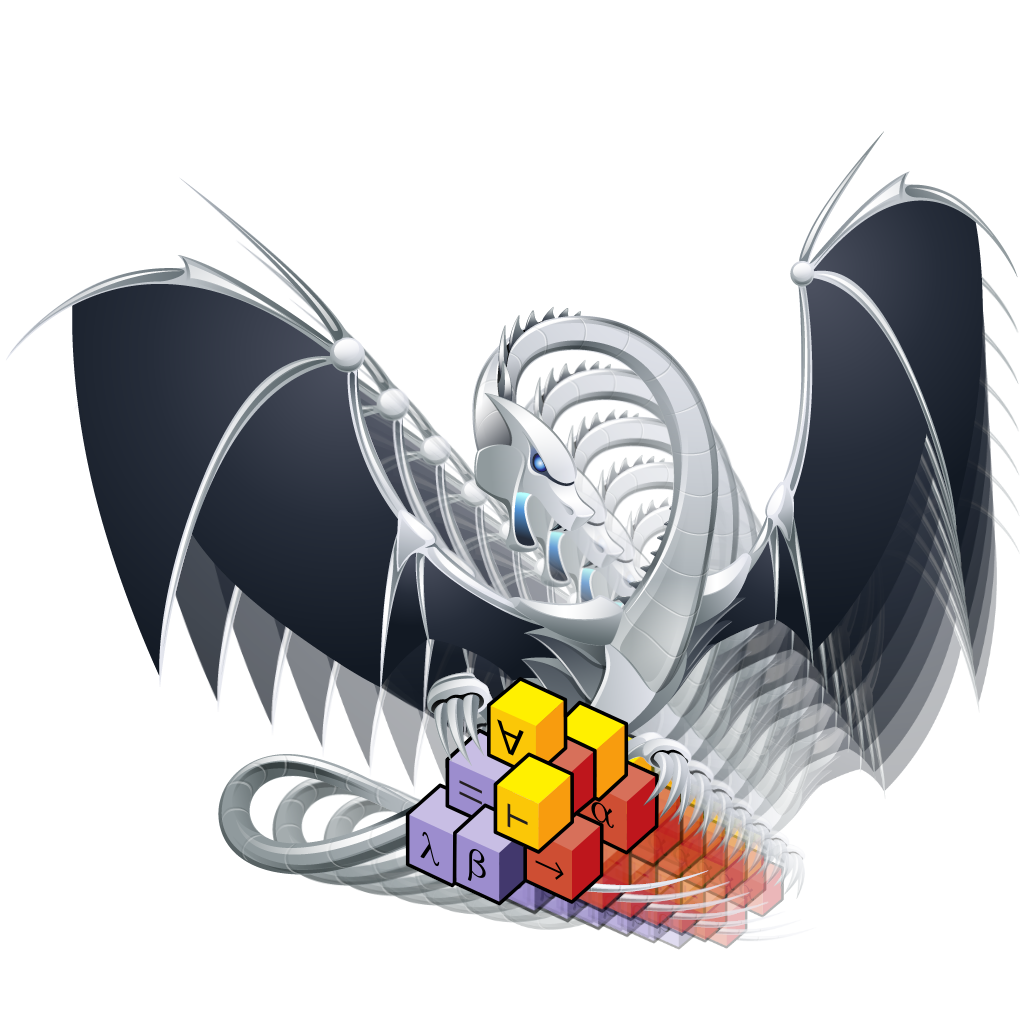
\includegraphics[height=\paperheight]{isabelle-llvm-par.png}};
% }
%
% # Conclusion
%   * Verification of parallel programs
%     * stepwise refinement to tackle complexity
%     * down to LLVM, small TCB
%     * \high{fast} verified programs
%
%   * Idea: shallow embedding, using access reports
%     * backwards compatible with sequential IRF
%
%   * Future work
%     * state-of-the-art parallel sorting
%     * fractional separation logic
%     * more concurrency
%     * complexity of parallel algorithms
%     * GP-GPUs
%
% }

\end{document}




